% Document Class
\documentclass[botnum, fleqn]{unmeethesis}


% Packages
\usepackage[dvipsnames]{xcolor}
\usepackage{listings}
\usepackage{rotating}
\usepackage{keyval}
\usepackage{fancyvrb}
\usepackage{xcolor}
\usepackage{float}
\usepackage{subcaption}
\restylefloat{figure}
\usepackage{ifthen}
\usepackage{calc}
\usepackage{ifplatform}
\usepackage{color}
\usepackage{rotating}
\usepackage[hidelinks]{hyperref}
\usepackage{algorithmic}
\usepackage[T1]{fontenc}
\usepackage{beramono}
% \usepackage[usenames,dvipsnames]{xcolor}



% Definitions
\definecolor{white}{rgb}{1.0,1.0,1.0}
\definecolor{lightgray}{rgb}{.9,.9,.9}
\definecolor{darkgray}{rgb}{.4,.4,.4}
\definecolor{darkcerulean}{rgb}{0.03, 0.27, 0.49}
\definecolor{purple}{rgb}{0.65, 0.12, 0.82}
\definecolor{darkred}{rgb}{0.55, 0.0, 0.0}

\lstloadlanguages{Ruby}
\lstset{
basicstyle=\ttfamily\color{black},
commentstyle = \ttfamily\color{red},
keywordstyle=\ttfamily\color{blue},
stringstyle=\color{orange}}


\lstdefinelanguage{JavaScript}{
  keywords={break, case, catch, continue, debugger, default, delete, do, else, false, finally, for, function, if, in, instanceof, new, null, return, switch, this, throw, true, try, typeof, var, void, while, with},
  morecomment=[l]{//},
  morecomment=[s]{/*}{*/},
  morestring=[b]',
  morestring=[b]",
  ndkeywords={class, export, boolean, throw, implements, import, this},
  keywordstyle=\color{blue}\bfseries,
  ndkeywordstyle=\color{darkgray}\bfseries,
  identifierstyle=\color{black},
  commentstyle=\color{purple}\ttfamily,
  stringstyle=\color{red}\ttfamily,
  sensitive=true
}

\lstset{
   language=JavaScript,
   backgroundcolor=\color{lightgray},
   extendedchars=true,
   basicstyle=\footnotesize\ttfamily,
   showstringspaces=false,
   showspaces=false,
   numbers=left,
   numberstyle=\footnotesize,
   numbersep=9pt,
   tabsize=2,
   breaklines=true,
   showtabs=false,
   captionpos=b
}

\lstdefinelanguage{JSON}{
  keywords={true, false, null},
  morestring=[b]",
  keywordstyle=\color{darkred}\bfseries,
  stringstyle=\color{darkcerulean}\ttfamily,
  sensitive=true
}

\lstset{
   language=JSON,
   backgroundcolor=\color{lightgray},
   extendedchars=true,
   basicstyle=\footnotesize\ttfamily,
   showstringspaces=false,
   showspaces=false,
   numbers=left,
   numberstyle=\footnotesize,
   numbersep=9pt,
   tabsize=2,
   breaklines=true,
   showtabs=false,
   captionpos=b
}

\lstdefinelanguage{Julia}
  {morekeywords={abstract,break,case,catch,const,continue,do,else,elseif,%
      end,export,false,for,function,immutable,import,importall,if,in,%
      macro,module,otherwise,quote,return,switch,true,try,type,typealias,%
      using,while},
   sensitive=true,
   % alsoother={$},
   morecomment=[l]\#,
   morecomment=[n]{\#=}{=\#},
   morestring=[s]{"}{"},
   morestring=[m]{'}{'},
}
[keywords,comments,strings]%

\lstset{
    language         = Julia,
    backgroundcolor=\color{white},
    basicstyle       = \ttfamily,
    keywordstyle     = \bfseries\color{blue},
    stringstyle      = \color{magenta},
    commentstyle     = \color{ForestGreen},
    showstringspaces = false,
}

% Begin Document
\begin{document}

% Frontmatter
\frontmatter

\title{Student Flow Simulation with Applications in Curricular Analytics}
\author{Michael Hickman}
\degreesubject{M.S., Computer Engineering}
\degree{Master of Science\\Computer Engineering}
\documenttype{Thesis}
\previousdegrees{B.S., University of New Mexico 2014}
\date{September, \thisyear}

\maketitle
\makecopyright


% % Dedication
% \begin{dedication}
%   Dedication goes here.
% \end{dedication}


% Acknowledgements
\begin{acknowledgments}
  \vspace{1.1in}
  I would like to thank ...
\end{acknowledgments}


% Abstract
\maketitleabstract

\begin{abstract}
  Abstract goes here
  \clearpage
\end{abstract}


% ToC and Figures
\tableofcontents
\listoffigures


% Glossary
\chapter{Glossary}
Discrete-Event Simulation
JSON
\mainmatter


%----------------------------------------------------------------------------------------
% INTRODUCTION
%----------------------------------------------------------------------------------------
\chapter{Introduction}
  The goal of every higher-education institution is to successfully educate students with skills and knowledge needed to enter, and be successful in the workforce. This is done by offering courses with desired learning outcomes required for success in a given field of work. These courses are then structured into a curriculum in which knowledge can be acquired and built upon. Moving students through these curricula is means in which universities and institutions achieve the goal of producing a student body well equipped for success in their chosen careers. Even more, universities are not merely just interested in students completing a program, but doing so in a timely manner. Most students wish to complete a degree as quick as possible and part of their success is determined by efficiency of their time at a university. Likewise, universities are incentivized to produce high four, five, and six year graduation rates.

  It is no surprise then that much time, money, and research are spent in attempts to improve timely student success and the efficiency of their offered programs. Examples include tutoring programs, better advisement, intervention programs, financial support, improving instruction quality, experimenting with classroom structures (hybrid courses, flipped classrooms etc.) and many more \cite{o2015use,topping1996effectiveness,hunter2004could,king2002identifying,lewallen1993early}. While these are all worthy pursuits that address many aspects of a student's academic career, there is one area that many universities often overlook when it comes to improving a student's journey through a curriculum: the structure of the curriculum itself.

  Every university's curricula are carefully designed and structured in such a way that students can achieve the learning outcomes defined for a given field of study. In most cases these learning outcomes are shared among most universities. The knowledge provided by a Mathematics at one university will most likely be the same as that at any other university. However, despite these shared learning outcomes every university's curricula is quite different. This is evident when viewing a curriculum as data - or more specifically, a graph, and by doing so the way in which it's structure can influence the efficiency of a student moving through it becomes apparent. For example see figure \ref{fig:comparison}.

  \begin{figure}
    \centering
    \begin{subfigure}[h!]{.6\linewidth}
      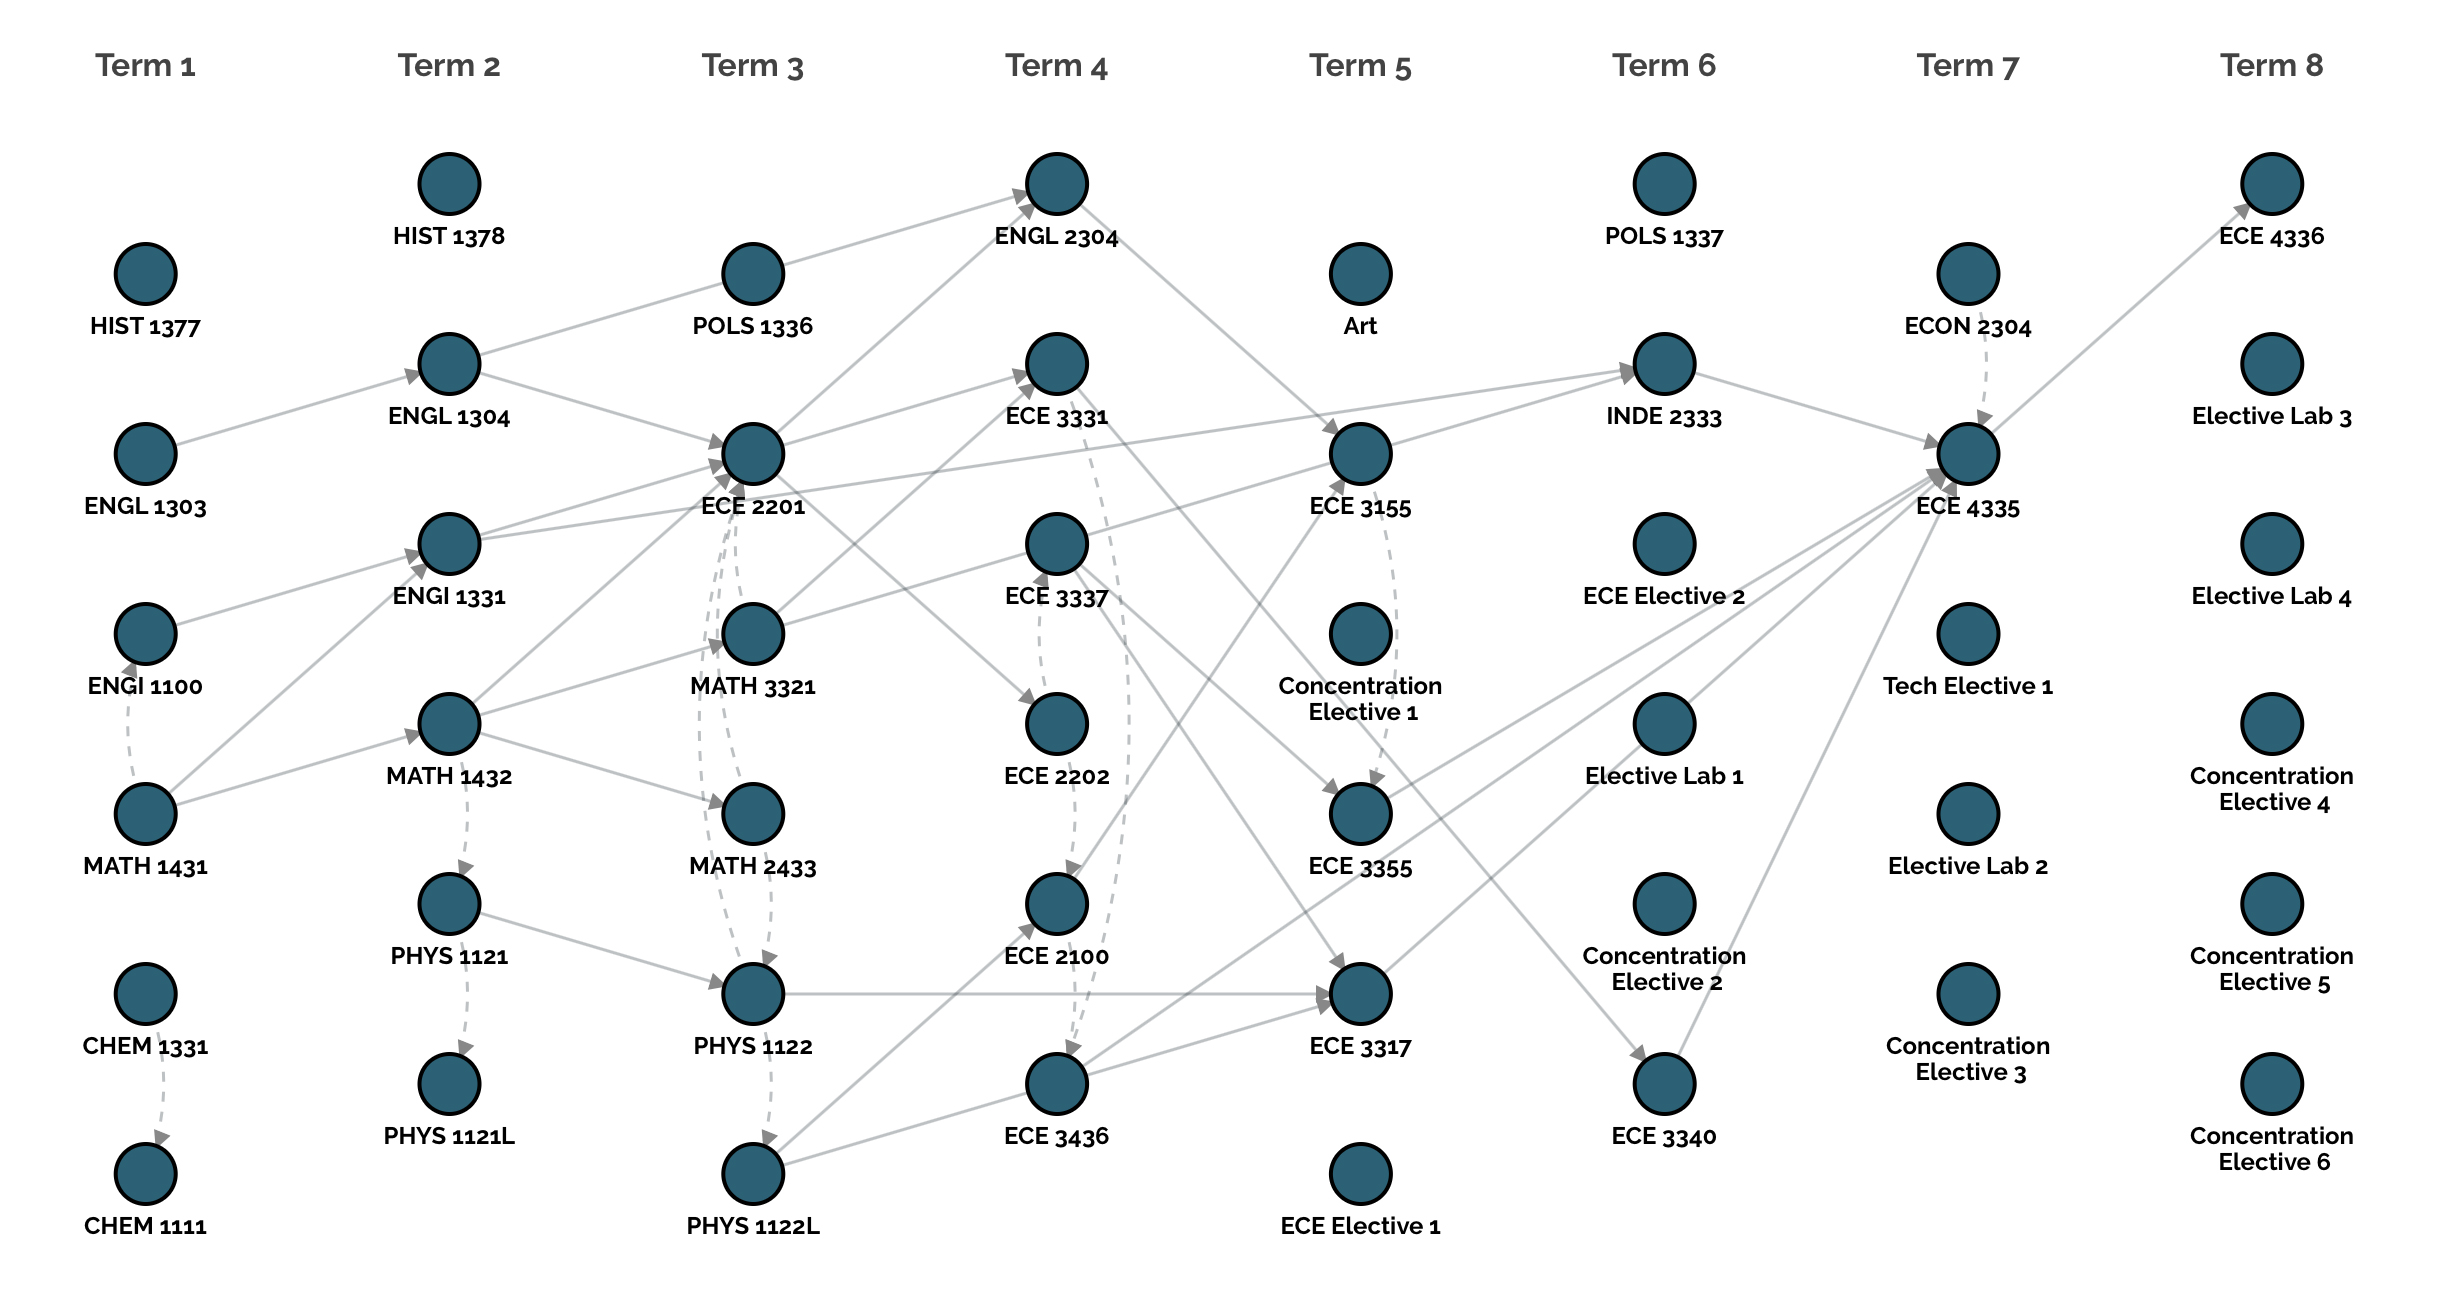
\includegraphics[width=\linewidth]{./figures/UH.jpg}
      \caption{University of Houston}\label{fig:UH}
    \end{subfigure}

    \vspace{1cm}

    \begin{subfigure}[h!]{.6\linewidth}
      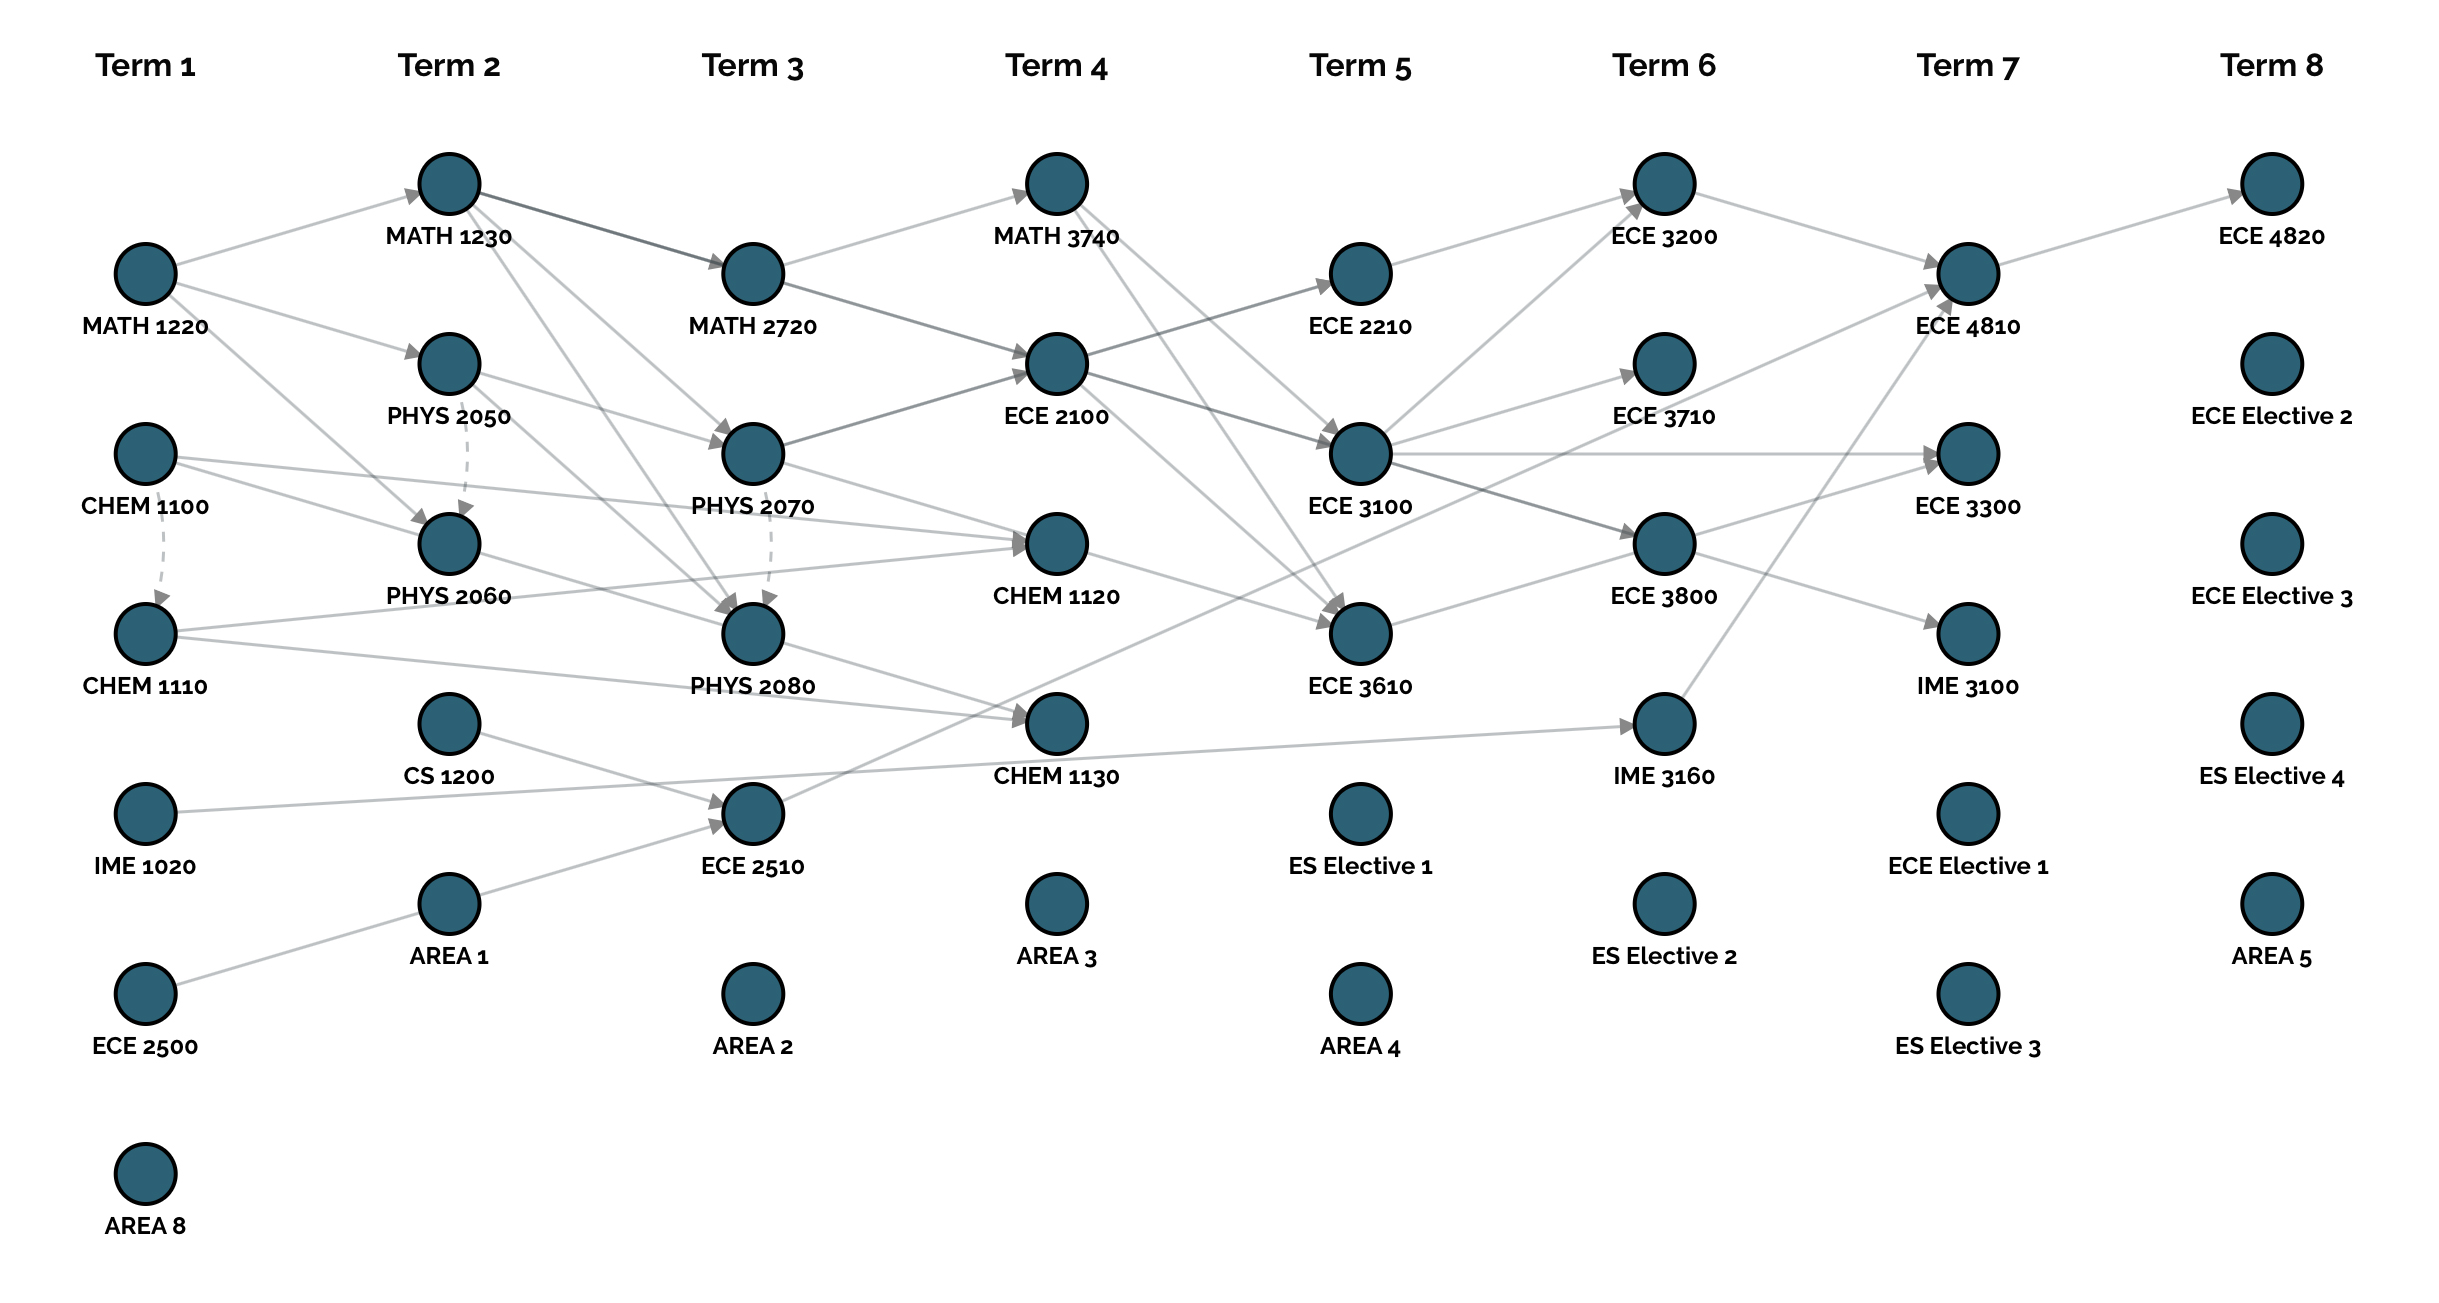
\includegraphics[width=\linewidth]{./figures/MU.jpg}
      \caption{Michigan University}\label{fig:MU}
    \end{subfigure}

    \caption{Comparison of two Electrical Engineering Curricula}
    \label{fig:comparison}
  \end{figure}

  In this figure you can see a comparison of two Electrical Engineering curricula from two different institutions. Figure \ref{fig:UH} shows University of Houston's while \ref{fig:MU} shows Michigan University's. Both curricula are four year programs within four credit hours of one another and even without knowing the specific courses in each it obvious that they are both structurally different from one another. This begs the question is one, based merely on structure alone, more conducive to timely graduation than the other?

  This thesis describes a software framework, the Curricular Analysis and Simulation (CAS) framework that allows for formal analytics over curricula to be done to help answer questions like the one previously posed. The framework described is an open-source Julia package that allows curricula to be represented in a programming, provides metrics for quantifying the complexity of a curriculum, both instructional and structural and, as it's name implies, simulates of students moving through curricula via discrete-event simulations. Though there are many statistical and machine-learning models for predicting the rate at which students might graduate, they fail to meaningfully represent the process from enrollment to graduation. This is where simulations can be a powerful tool for understanding not just how fast, but how students move through curricula and how curriculum characteristics play a role. This, rather than accurately predicting completion rates is the main focus of the CAS framework.


%----------------------------------------------------------------------------------------
% Previous Work
%----------------------------------------------------------------------------------------
\chapter{Previous Work}

  \section{Defining Structural Complexity}
    Before being able to determine the effects a curriculum's structure has on the ease in which students can move through it, it is necessary to quantify the structure, or rather the complexity of a curriculum's structure. A team of researches at the University of New Mexico have done just that by introducing two metrics that attempt to capture properties of a curriculum structure that pertain to a students progressing though it \cite{complexity}. As previously seen in figure \ref{fig:comparison}, a curriculum can be represented as a graph allowing it to be subject to graph theory and complex network analysis, which serves as the basic of UNM's work. Computing this metric, which is simply called the \textit{structural complexity} of a curriculum, begins by assigning each course a value, called its \textit{course cruciality}, which signifies how important the course is in the curriculum. This value is in turn comprised of two other measures: the course's \textit{blocking factor} and it's \textit{delay factor}.

    A course's delay factor is defined as the number of nodes (or courses) on the longest path that passes through the given course. An example can be seen in figure \ref{fig:delay_factor_example}. In this figure, course A has a delay factor of three as the longest path that passes through it contains three courses: A, B, and D, as opposed to the short path with length two that contains courses A and C. Course B and D share course A's delay factor of three, while course C only has a delay factor of two.

    \begin{figure}[h!]
      \centerline{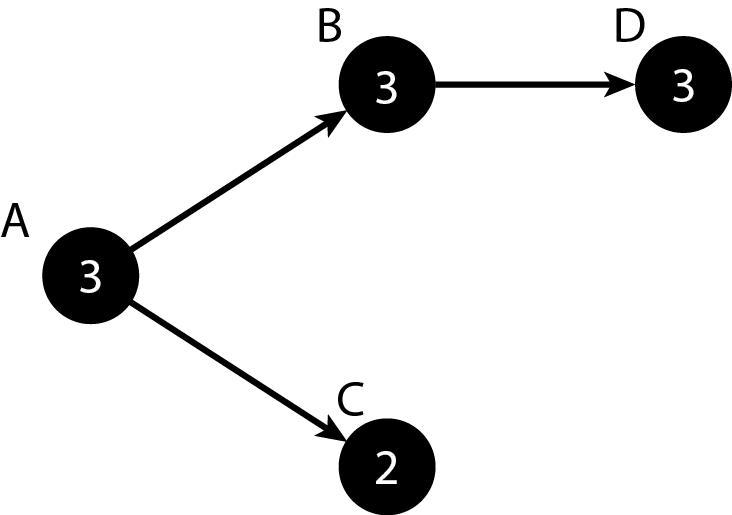
\includegraphics[scale=0.4]{./figures/delay_factor.png}}
      \caption{Delay factors are given for courses A, B, C, and D.} 
      \label{fig:delay_factor_example}
    \end{figure}

    A course's blocking factor is defined as the number of courses that are blocked from being taken if the given course is not passed. This is essentially the connectivity of the course. If there is a path from node \(i\) to \(j\) then \(n_{ij}\) is 1 and 0 otherwise. Then, the blocking factor of course i would be given by:

    \begin{equation}
      V_{i} = \sum_{j} n_{ij}
    \end{equation}

    An example of blocking factors can be seen in figure \ref{fig:blocking_factor_example}. Here, course A has a blocking factor of three because it is connected (or blocks) three other courses: B, C and D. Course B blocks one course, D and course C and D have a blocking factor of zero because no courses succeed them.

    \begin{figure}[h!]
      \centerline{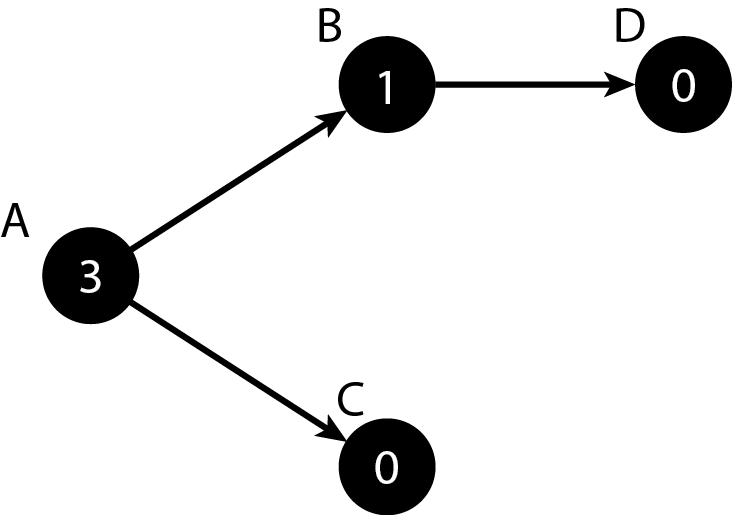
\includegraphics[scale=0.4]{./figures/blocking_factor.png}}
      \caption{Blocking Factors are given for courses A, B, C, and D.} 
      \label{fig:blocking_factor_example}
    \end{figure}

    Given a course delay factor \(L_i\), and blocking factor, \(V_i\), then it's cruciality, \(C_i\) is simply given by the sum of the two:

    \begin{equation}
      C_{i} = V_{i} + L_{i}
    \end{equation}

    A curriculum's complexity, \(S\) is then given by the sum over all course crucialities:

    \begin{equation}
      S = \sum_{i}^n C_{i}
    \end{equation}

  \section{Student Simulations}
  TODO: DESCRIBE PAPERS ON SIMULATING STUDENTS.

%----------------------------------------------------------------------------------------
% Simulation
%----------------------------------------------------------------------------------------
\chapter{Simulating Students in a Curriculum}

  \section{Discrete Event Simulations}
  Students moving through a curriculum can be viewed as a fixed, chronological sequence of events. Students will enter the university, enroll in classes, complete or withdraw from classes, then graduate if all requirements have been met. This process repeats every semester. Discrete-event simulation models a system by emulating a sequence of events, where every event occurs independently of the others at a particular instance in time and are characterized by having the following components:

  \begin{itemize}
  \item \textbf{Starting and Ending States} - The simulation will begin in a given state and will continue until it reaches another state that represents some pre-defined ending-condition or a point in time.
  \item \textbf{Clock} - The simulation must keep track of the time that has ellapsed after it begins in any time unit relevant to the domain of the simulation. The clock does not run continuously as events occur instantaneously, but it does jump to certain times as events occur.
  \item \textbf{List of Events} - The system maintains a list of events that can occur during the simulation. These events are placed in a que and are usually executed based on simulation time rather than the time they were queued.
  \item \textbf{Statistics} - As the ending state is not the only result of interest when running simulations, the system keeps track of various statitics based on the events that have occured.
  \end{itemize}

  Using these components, a simulation is constructed using the basic following logic:

  \begin{algorithmic}[1]
  \STATE Initialize the system
  \STATE Initialize the system clock
  \STATE Schedule the initial event
  \WHILE{ending condition is false} 
    \STATE{Increment clock}
    \STATE{Perform next event}
    \STATE{Update system statistics}
  \ENDWHILE
  \STATE Output simulation results
  \end{algorithmic}

  Given these characteristics and basic logic flow, this type of simulation lends itself well to the process of students flowing through a curriculum within an institution, much more so than continuous-time simulations and other analytical models; therefore, the student-flow simulation is modeled as a discrete-event simulation.

  \section{Defining A Curricula}
  A curriculum is the backbone of the simulation. As the goal of the simulation is to model students moving through a curriculum, the events of the simulation depend on the curriculum that is being simulated; therefore it is important to understand how they are defined. In order for a student to obtain a degree within a given academic program, a set of requirements must be met. The requirements, in most cases, are simply courses that must be passed. However a curriculum is more than a set of courses, but rather an arrangement of courses with constraints as to when they can be taken. This arrangement begins by placing courses within terms where, ideally, student would take and pass the entire set of courses in one semester. Next, relationships are created between courses in the form of prerequisite and co-requisite relationships. This structure of courses grouped in terms with defined relationships make up a curriculum. A visual, graph representation of a curriculum can be seen in Figure \ref{fig:curriculum_example}.

  \begin{figure}[h!]
  \centerline{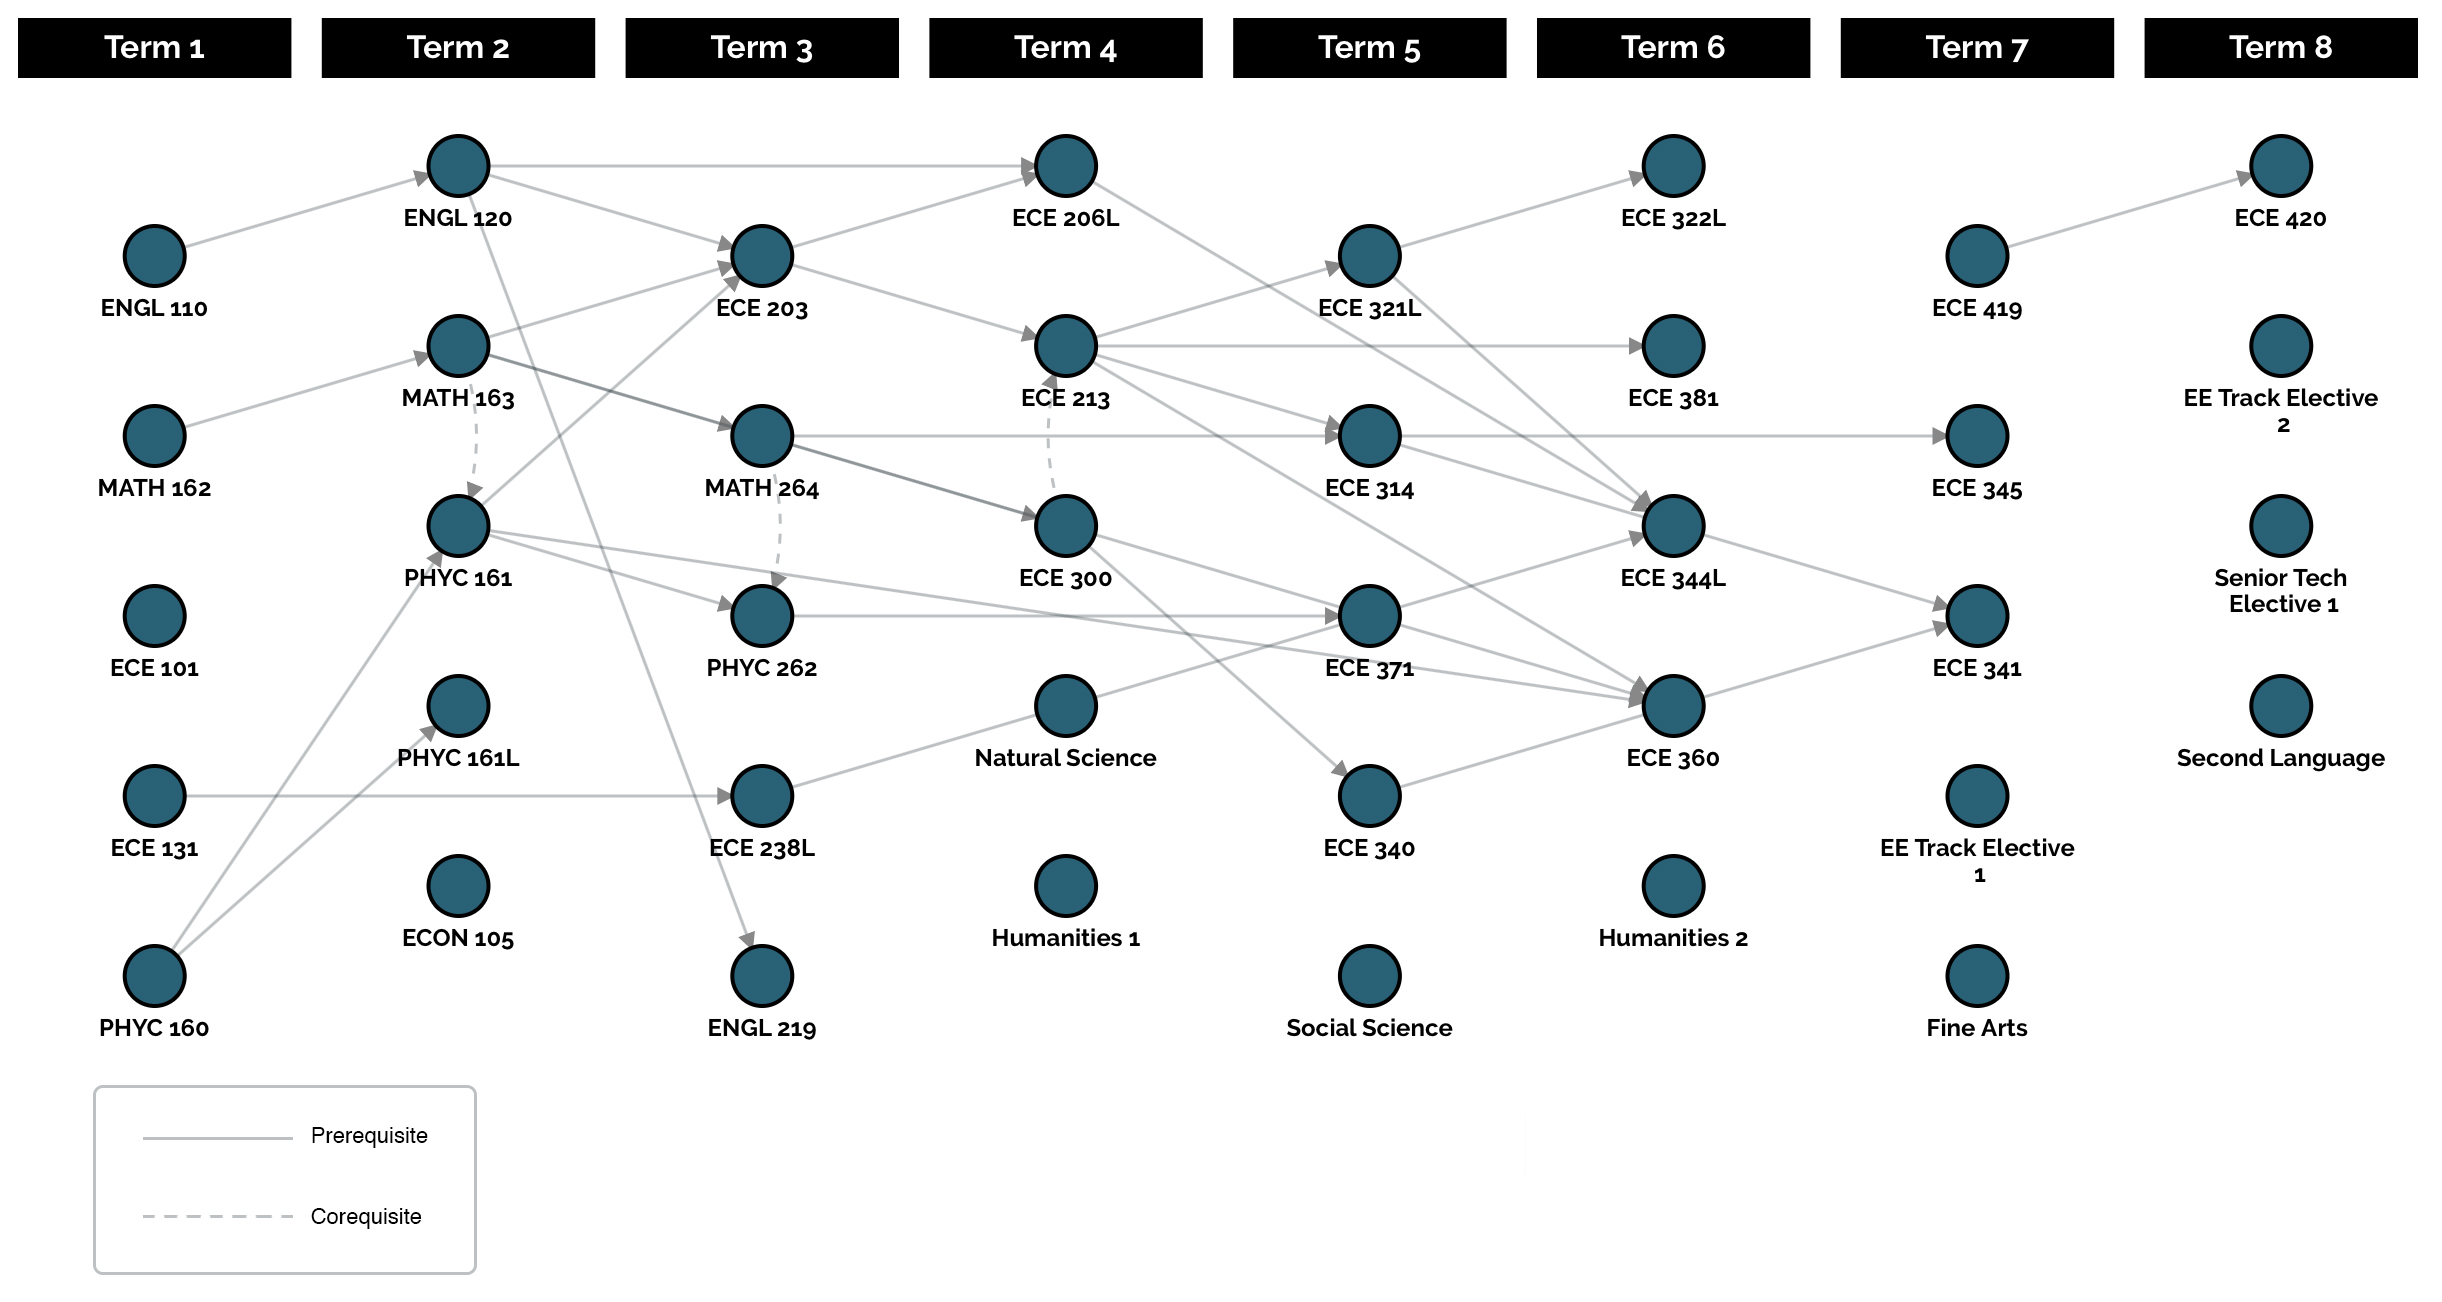
\includegraphics[scale=0.4]{./figures/curriculum_example.jpg}}
  \caption{Visual representation of the electrical engineering curriculum at UNM.} 
  \label{fig:curriculum_example}
  \end{figure}


  \section{Assumptions}
  A student's academic career within an institution can potentially be a very difficult thing to model. This is primarily because student behavior can be erratic and unpredictable even given a structured curriculum. Students might not register for the courses they should, take courses that don't count, drop classes, take a semester off, get an override to take a course that they normally wouldn't have been able to, and various other actions that would otherwise not be considered \'typical' behavior. There are a vast amount of factors that can influence student behavior, many of which are not academic and would therefore be very difficult to account for. Furthermore universities can impose various policies that would also have an effect on how students register for classes and affect other academic decisions. 

  Trying to realistically simulate all possible actions that a student can take would be impossible, therefore several assumptions and decisions are made to simplify student behavior down to the basics, making meaningful simulation feasible without needless complexity. The most influential decisions made, was to design the student flow simulation with the primary goal of performing analytics over curricula and observing the effects their properties have on students moving through it. This is in contrast to developing a system to provide realistic simulations of student behavior with the goal of predicting graduation rates and other statistics. The simulation is potentially capable of this; however it was not the goal. Thus the other decisions made were done so to put emphasis on how curricula influence outcomes relative to one another instead of how student behavior does so. Below is a list of the other assumptions and decisions:

  \begin{itemize}
    \item All students at the beginning of the simulation are treated as first-time, full-time students. Although in many cases actual freshman might have some college credit, either through AP-tests, taking college-classes while in high-school, or transfers, students in the simulation begin with a clean slate. They are also treated as full-time students with no notion of \'part-time' built in.
    \item Given that all students are full-time, each semester all students will register for as many credits as they can. In reality, most students do not hit their institutions max credit-hour limit, but the simulation will register students in as many courses as they are allowed - which is set by the user.
    \item The simulation only deals with a single class of admitted students. There is no continuous influx of freshman or transfer students each semester within the simulation.
    \item Students who stop-out are dis-enrolled permanently. They do not re-enroll.
    \item Students will only register for courses within the specified curriculum. The simulation is only aware of the courses specified in the curriculum, so while it is common for students to register for courses that might not count towards their major, this behavior is not part of the simulation.
    \item The order of courses in which students enroll in depends on their ordering within the curriculum. Students will enroll is the earliest listed course within the curriculum and will roll in each course they can as until they hit the credit-hour limit. This process is described in greater detail later.
    \item The minimum passing grade is universal among all courses. This grade can be set by the user, and defaults to a C-.
    \item All course enrollment requirements are strictly enforced. While it is common for students to obtain permission and subsequent overrides to enroll in a class they have not met the requirements for, the system does not allow for this.
    \item All courses within a curriculum are offered every semester.
    \item Courses have no notion of capacity. Any number of students can be enrolled in any course in a given term.
  \end{itemize}

  These decisions might seem very restrictive, and in many ways that is intentional. The idea wasn't to simplify the simulation for the sake of simplicity, but rather to put more emphasis on the curriculum and its structural properties. By standardizing the way students behave, it is possible to compare curricula and how changes to their structure or difficulty effect outcomes which provides insight into how they might be improved.

  \section{Simulation Model Logic}
  The student flow simulation uses the components and basic logic of DES previously described and adapts them to fit within the domain of students flowing through a curriculum. The components are defined as follows:

  \textit{Clock}. The unit of time in which the simulation uses is a semester. All events occur within one semester, therefore the clock will on increment time by one semester.

  \textit{Starting State}. The simulation begins with a set of students which represent first-time full-time students just enrolled in a university. The clock is set to the first semester.

  \textit{Events}. The primary events in the simulation emulate basic student behavior during their academic career:
  \begin{itemize}
    \item Students enroll in the university.
    \item Student enrolls in the courses that they are able to take.
    \item Student takes the classes they enrolled in and are assigned a grade, either passing or failing.
    \item Student stopouts.
    \item Student graduates.
    \item Student remains enrolled.
  \end{itemize}

  \textit{Ending Condition}. The simulation ends when there are no students enrolled. Therefore all students have either graduated or stopped out. The simulation could end before this however as it can also be run for a set amount of semesters.

  \textit{Statistics}.

  \subsection{Control Flow}
  The simulation begins at its starting state - a set of students with no previous academic experience and a clock set to semester one. Each student is initiated with defined attributes. All enrolled students then begin registering for classes using a systematic approach governed by the way the curriculum is defined. The order of the courses in the curricula governs the order in which students register. Students will always register for the earliest courses listed within the curricula and continue registering for courses until there are no more courses that they can take or they cannot register for more courses due to the given term credit hour restriction. For example, if the first term within a curriculum consists of courses A, B, and C, the student will register for those courses in that order. If the students fails course B, then the following term, this will be the first course the student enrolls in. In order for a student to register for a course, they must meet the course's enrollment requirements. These requirements can be prerequisites, co-requisites, a term restriction meaning that the course cannot be taken until the clock reaches a specified term, and that the student has not already taken and passed the course. In addition to these requirements, a student can only register for so many courses in a given term based on a given maximum credit hour limit which is set by the user. If a student can register for a course then they are added to that course's list of enrolled students and their term credit hour count is incremented by that courses credit hour value. 

  Once all students have completed the registration process, every student is assigned a grade for the courses they are enrolled in. The method for doing so depends on the user and will be covered later. The simulation uses the following grades: A+, A, A-, B+, B, B-, C+, C, C-, D+, D, D-, F, and W. The system also assigns numeric values to each grade which are 4.33, 4.0, 3.77, 3.33, 3.0, 2.77, 2.33, 2.0, 1.77, 1.33, 1.0, 0.77, 0 and 0, respectively. These values are used for GPA computations, point calculations, and can possibly be used to determine grades in other courses. The passing grade can be set by the user, but defaults to a C (2.33). If a student obtains this grade then their completion of the course is recorded.

  Once all students have received their grades for all courses, the students GPA's are computed and then the simulation will check to see if each student has completed all requirements in the curriculum. If they have, then they are removed from the pool of enrolled students and added to the list of graduated students. They system will then simulate students stopping out. Again, the user can determine the method used for doing this which will be explained later. If the student is chosen as a stopout, then they are removed from the pool of enrolled students and added to a list of stopped out students. The clock is then incremented by one semester and the registration process begins for the next semester. These events are then repeated until there are no students enrolled, or the simulation clock reaches a time set by the user.


%----------------------------------------------------------------------------------------
% Curricula Simulation Framework Design
%----------------------------------------------------------------------------------------
\chapter{Curricula Simulation Framework Design \& Implementation}

  \section{Julia}
    The CAS framework is implemented in the open-source Julia programming language and made available as an open-source Julia package. Julia is described as a high-level, high-performance dynamic programming language for technical computing that "has the performance of a statically compiled language while providing interactive dynamic behavior and productivity like Python, LISP or Ruby" \cite{Julia}. It is built upon an LLVM-based just-in-time (JIT) compiler which allows it to reach performance close to that of C and, in many cases, speeds faster than that of R or MATLAB \cite{Julia}. Julia's defining feature is multiple dispatch but some other notable features are module support, a type system, parallelism and a built-in package manager. It also has a thriving community of developers contributing high-quality open source libraries spanning a range of applications such as machine-learning, statistical analysis, graph analysis, plotting, and data-handling.

    Each of these features contributed to choosing Julia as the language of implementation. Julia's type system, ease of use and dynamic nature made it simple to implement the framework's various components, methods logic. Working with data formats such as JSON and CSV were especially easier that a computation language such as MATLAB. However this ease of development did not come at the expense of performance as Julia is incredibly fast and it's support for parallelism allowed running many simulations much faster as they could be carried out in parallel. Topping it all off is it's built in package manager with a plethora of packages that will enable uses extend the framework and simulation capabilities with powerful machine learning and statistical models.

  \section{Architecture and Implementation Details}
    The framework is comprised of three main components: (1) custom data types, (2) the simulation method, and (3) course performance prediction modules. The first component, a set of custom data types, represent all the necessary components (curricula, students, etc.) over which analysis and simulations can be performed. The second component of the framework is a method that carries out a simulation using a defined curriculum and a set of students taking into account various simulation parameters that can be set by the user. The third and final component of the framework are.\ modules which are passed into the simulation method that determine how the virtual students 'perform' in each course. The framework comes with one out of the box, but users can develop their own to conduct simulations that suite their needs. A system diagram can be seen in figure \ref{fig:component_diagram}. The next several sections describe each component in greater detail.

    \begin{figure}[h!]
      \centerline{\includegraphics[scale=0.4]{./figures/component_diagram.jpg}}
      \caption{A component diagram of the CAS framework.} 
      \label{fig:component_diagram}
    \end{figure}

    \subsection{Framework Data Types}
      Custom Julia types serve as the foundation of the framework allowing curricula and related entities to be defined a mutable objects allowing analysis and simulation to be performed. These data types are: curricula, terms, courses, students, and simulations. Due to Julia not being an OO language, these entities are not true objects, but are very similar to structures in C in that they do not have associated methods, but do have associated attributes. Each type's attributes describe the characteristics of the entity it represents as well as provides a place to record statistics regarding the entity after a simulation is performed.

    \subsubsection{Course Type}
      At the heart of every curriculum are courses and every course in a curriculum is represented by its own object. These objects have the following attributes:

      \begin{description}
        \item [name] A string that is used to identify the course. This can be anything, but the best options would a course code, such as 'MATH 162' or the course's title such as "Calculus I".
        \item [id] A unique integer identification number for the course.
        \item [credits] The number of credit hours the course is worth.
        \item [delay] The course's delay factor.
        \item [blocking] The course's blocking factor.
        \item [cruciality] The course's cruciality.
        \item [prereqs] An array of courses that are considered prerequisites.
        \item [coreqs] An array of courses that are considered co-requisites.
        \item [postreqs] An array of courses that the courses is a prerequisite or co-requisite to.
        \item [termReq] A courses minimum term requirement. For example, if this value is 2, then the courese could not be taken until at least the second term.
        \item [students] An array of students that are enrolled in the courses in a given term. The simulation populates this array each term, and then at the end of the term, empies it.
        \item [passrate] The course's actual, real-world pass-rate. This is a percentage of students that pass the course represented as a floating point number between 0 and 1.0, where 1.0 is a 100\% pass-rate.
        \item [failures] The number of simulated failures. Every time a student within the simulation fails the course, this value is incremented.
        \item [grades] An array of all simulated grades made by students enrolled in the course.
        \item [enrolled] The total number of students enrolled in the course over the course of the simulation.
        \item [termenrollment] An array of the number of students enrolled in the course each term. For example an array of [20, 30, 25] indicates that 20 studets were enrolled in term one, 30 students in term two and 25 students in term three.
        \item [termpassed] An array of the number of students who passed the course each term.
        \item [model] A julia dictionary, which is an associative array, that is used to store any kind of data pertaining to the prediction model the user selects for making grade predictions for students enrolled in the course. A dictionary was chosen because it is extremely flexible in terms of the values it can store and therefore suitable when the types of stored information is unknown prior to runtime.
      \end{description}

      Like all types in Julia, a course object is instantiated via a constructor method that has the same name as the type. Unlike other languages, Julia allows a type to have multiple constructors and in this case, the course type has four. Each constructor has the same name, \textit{Course()}, but the number and types are arguments differ. All constructors require a name, the number of credits the course is worth, an array of prerequisites and and array of co requisites with one of the constructors accepting only these arguments. The others constructors allow more information to be provided, specifically a pass-rate, a termReq, or both. Examples of the constructors can be seen below.

      \lstinputlisting[language=Julia, basicstyle=\tiny, numberstyle=\tiny, xleftmargin=0.65cm, xrightmargin=0.55cm]{code/course_constructors.jl}

    \subsubsection{Term Type}
      The term type essentially represents a collection of courses that, ideally, would be taken together in the same semester. It has the following attributes:

      \begin{description}
        \item [courses] An array of courses that make up the term. The order of the courses matters, as those that are at the beginning of the list will be registered for first.
        \item [credits] The sum of the credit hour values of courses within the term.
        \item [totalEnrolled] The total number of students enrolled in the courses that belong to the term.
        \item [failures] The total number of failing grades made in the courses that belong to the term.
      \end{description}

      The term type only has a single constructor that accepts an array of courses:

      \lstinputlisting[language=Julia, basicstyle=\tiny, numberstyle=\tiny, xleftmargin=0.65cm, xrightmargin=0.55cm]{code/term_constructors.jl}

    \subsubsection{Curriculum Type}
      The curriculum type brings the term and course types together to define a complete academic program that contains a structured set of courses that students must progress through to obtain a degree. This is the type that the framework uses to perform a simulation over a curriculum. It has the following attributes:

      \begin{description}
        \item [name] A string identifier for the curriculum.
        \item [terms] An array of terms that make up the curriculum. The order should reflect the actual order of the terms.
        \item [courses] An array of all the courses within the curriculum. This array is created from the array of terms and serves as a more convenient way to access the curriculum's courses rather than having to access them through the terms array.
        \item [numCourses] The number of courses in the curriculum.
        \item [complexity] The curriculum's complexity.
        \item [delay] The sum of the courses' delay factors.
        \item [blocking] The sum of the courses' blocking factors.
        \item [passrate] The average of the curriculum's courses' real-world pass-rates. Can be used as a naive measure of difficulty.
        \item [stoupoutModel] A dictionary that stores the model that predicts student stopouts.
      \end{description}

      The curriculum has two constructors. The first takes a string that represents its name and an array of terms as arguments. The issue with this constructor, although it is completely usable, is that it requires the term objects, and therefore course objects to already be instantiated. This can be a tedious and time consuming and is not a very good way to store curricula in a extensible format. To address this problem, a JSON file format was developed as a straightforward way to define a curriculum that is easier to create, more portable, as well as easier for a computer to generate or read.

      At the root of this definition is an object with two keys: \textit{terms} and \textit{courses}. The \textit{terms} key stores the number of terms in the curriculum. The \textit{course} key stores an array of objects that represent a course. These objects have the following keys: \textit{name}, \textit{credits}, \textit{passrate}, \textit{term} which is the term the course belongs to, \textit{prerequisites} which is an array of strings corresponding to the names of the course's prerequisites, and \textit{co-requisites} which is an array of strings corresponding to the names of course's co-requisites. An example can be seen below:

      \lstinputlisting[language=JSON, basicstyle=\tiny, numberstyle=\tiny, xleftmargin=0.65cm, xrightmargin=0.55cm]{code/sample_curriculum.json}

      The second constructor method accepts a name and another string that is expected to be a path to one of these JSON files. The method will parse the file and create course and term objects automatically. This makes it much more convenient to create a curriculum object along with objects for its associated courses and terms. Below are examples of these constructors:

      \lstinputlisting[language=Julia, basicstyle=\tiny, numberstyle=\tiny, xleftmargin=0.65cm, xrightmargin=0.55cm]{code/curriculum_constructor.jl}

    \subsubsection{Student Type}
      Every student in the simulation is represented by its own student object. Therefore, the student type was designed to contain all the information needed to track a student's progress as well as represent the characteristics that define the student and aid in grade predictions. It was designed to be flexible allowing the user to determine what characteristics are needed rather than have a set of hard-coded attributes. The attributes for the student type are:

      \begin{description}
        \item [id] A unique integer identifier for the student. Before a simulation is run, these are set to ensure all student ids are unique integer values starting at one.
        \item [total\_credits] The total number of credit hours a student has earned during the simulation.
        \item [total\_points] The total number of points a student has earned during the simulation. The number of points a student earns for a course is the product of the number of credit hours for the courses and the received grade's value. For example if a student earns a B+ in a three credit hour course, then they will receive (3.3*3) or 9.9points.
        \item [gpa] The students grade point average, which is computed at the end of every term. It is derived by dividing the student's \textit{total\_points} by their \textit{total\_credits}.
        \item [termcredits] The number of credit hours the student registers for in a single term. At the end of every term it is reset to zero.
        \item [stopout] A boolean value that indicates whether a student has stopped out and is no longer enrolled.
        \item [stopsem] The term in which a student stops out.
        \item [graduated] A boolean value that indicates whether a student has graduated.
        \item [gradsem] The term in which the student graduates.
        \item [performance] A dictionary that keeps track of how students perform in the classes they enroll in. The key value pair consist of the course name and letter grade made, respectively.
        \item [attributes] A dictionary that stores the student's characteristics. What the exact attributes are is up to the user to decide and is most likely based on the variables to predict or assign grades. For example if the grade prediction model uses high school GPAs and ACT scores as features, then these attributes will be stored here.
      \end{description}

      The student type only has one constructor which simply takes a dictionary of student attributes as an argument. Below is an example:

      \lstinputlisting[language=Julia, basicstyle=\tiny, numberstyle=\tiny, xleftmargin=0.65cm, xrightmargin=0.55cm]{code/student_constructor.jl}

    % *** 

    \subsubsection{Simulation Type}
      A simulation object is used to store the results of a simulation, as well as tie all of the individual pieces together so they can be easily accessed through a single object. The curriculum, students, and results are all contained within this object. This makes it easy to keep track of all the data used in a simulation as well as compare multiple simulations. This type has the following methods:

      \begin{description}
        \item [curriculum] A curriculum object to be simulated.
        \item [duration] The number of terms the simulation ran for.
        \item [predictionModel] A Julia module that implements the model used for predicting student outcomes in each class.
        \item [numStudents] The number of students that participate in the simulation.
        \item [enrolledStudents] An array of students that are still enrolled when the simulation ends.
        \item [graduatedStudents] An array of students that have graduated during the simulation.
        \item [stopoutStudents] An array of students that stopped out during the simulation.
        \item [studentProgress] A \textit{courses x students} matrix that is used keep track of which students have passed which classes. Each row is associated with a student and each column a course. The indices of each column and row match the id's of their associated student and course. A value of 1 in the matrix indicates that the row's associated student has passed the column's associated course, while a 0 indicates that the course has not been passed by the student.
        \item [gradRate] The simulated graduation rate at the end of the simulation.
        \item [termGradRate] An array that contains the simulated graduation rates at the end of each term.
        \item [stopoutRate] The stopout rate at the end of the simulation.
        \item [termStopoutRates] An array that contains the stopout rates at the end of each term.
      \end{description}

      Before any simulation, a simulation object is created that contains a curriculum and an optional Julia grade prediction module. If no module is passed in then a default is used. It has a single constructor shown below:

      \lstinputlisting[language=Julia, basicstyle=\tiny, numberstyle=\tiny, xleftmargin=0.65cm, xrightmargin=0.55cm]{code/simulation_constructor.jl}

  %----------------------------------------------------------------------------------------
  
  \subsection{Performance Modules}
    Performance modules are used to predict the grades that students make in their enrolled courses. These modules give users the ability to specify exactly what kind of prediction model they would like to use, although they must implement it themselves. Given the number of open-source Julia regression and machine learning libraries available, a wide variety of techniques can be easily implemented. This makes the simulation framework flexible and allows it to cary out a wide variety of simulations so that users can find the one that best fits their data. 

    A performance module is simply a Julia module that contains three functions: \textit{train()}, \textit{predict\_grade()}, and \textit{predict\_stopout}. These methods are used during the simulation, and do not need to be called by the user manually, therefore it is important that they are implemented correctly. The \textit{train()} method is called before the simulation begins and performs any kind of training that might be necessary for predictions, accepting a single curriculum object as a parameter. This gives the user access to all of the courses, where some sort of prediction model will be trained for each one based on features that the user has selected and will be included in the student's attributes. Of course these trained models will need to be stored somewhere and that's why each course has a \textit{model} attribute. This attribute is a dictionary that can store any kind of data. The user can take advantage of this to store any information or objects relevant to the model for each course. Also, a model for predicting whether or not a student drops out must be trained. Like the course's \textit{model} attribute, the curriculum's \textit{stopoutModel} attribute will store any relevant information. Below is a template function:

    \lstinputlisting[language=Julia, basicstyle=\tiny, numberstyle=\tiny, xleftmargin=0.65cm, xrightmargin=0.55cm]{code/train.jl}

    The next function, \textit{predict\_grade()}, actually predicts a grade for a student. It takes in two arguments: a course object and a student object. Because the model for the passed in course object has already been trained, then the course's \textit{model} contains the necessary information to construct the model and the student's \textit{attributes} contain the features used in the model making it possible to predict a grade. As mentioned previously, grades are represented by floating point numbers that correspond to a letter grade, therefore a numeric value is expected to be returned. An example can be seen below:

    \lstinputlisting[language=Julia, basicstyle=\tiny, numberstyle=\tiny, xleftmargin=0.65cm, xrightmargin=0.55cm]{code/predict_grade.jl}

    The last function in the performance module, \textit{predict\_stopout()}, takes a student object, the current term, and the curriculum's \textit{stopoutModel} attribute as arguments and predicts whether or not a student will stop out. This process is similar to the grade prediction: the model is constructed and given the student's features a prediction will be made. This prediction should return either true, meaning the student drops out, or false indicating that the student remains enrolled. See example below:

    \lstinputlisting[language=Julia, basicstyle=\tiny, numberstyle=\tiny, xleftmargin=0.65cm, xrightmargin=0.55cm]{code/predict_stopout.jl}

    Once a user constructs one of these modules, they will specify that they would like to use when they create a simulation object. However, if no module is passed in a default module built into the framework will be used. This default model simply uses the pass-rate of a course as a probability of passing a course. This model doesn't so much predict a grade as a it does predict whether a student will pass a course by carrying out a single Bernoulli trial. A 'success' is interpreted as a student making an 'A' and a 'failure' results in the student receiving a 'F'. A Bernoulli trial is also used to determine stopouts, where the probability of stopping out is based on the current term and it's corresponding real-world retention value at UNM. Below is the code for this module:

    \lstinputlisting[language=Julia, basicstyle=\tiny, numberstyle=\tiny, xleftmargin=0.65cm, xrightmargin=0.55cm]{code/PassRate.jl}

  %----------------------------------------------------------------------------------------
  
  \subsection{Simulation Method}
    All of the components that have been described come together to perform what the Curriculum Flow framework was designed to do - simulate students flowing through a curriculum. This simulation is carried out through the framework's \textit{simulate()} method. This method requires two arguments: a simulation object, and an array of students. It will also accept three optional arguments: \textit{max\_credits}, \textit{duration}, and \textit{stopouts}. The first, \textit{max\_credits}, allows the user to specify the maximum number of credit hours that a student can take in a given term. If no value is specified then the simulation defaults the value to 18. To specify how long the simulation will run for, the \textit{duration} argument can be set. The simulation will run for the specified number of terms as long as there remails enrolled students. The default value is 8. The \textit{stopouts} argument is a boolean value that tells the simulation whether to include stopout students. If false, then no students will ever stop out, while a true value will use the Performance Module's \textit{stopout()} method to unenroll students at the end of every term. An example of how all these pieces come together to run a simulation is shown below:

    \lstinputlisting[language=Julia, basicstyle=\tiny, numberstyle=\tiny, xleftmargin=0.65cm, xrightmargin=0.55cm]{code/sample_simulation.jl}


%----------------------------------------------------------------------------------------
% Application
%----------------------------------------------------------------------------------------
\chapter{Application in Curricular Analytics}

  \section{Correlating Complexity with Completion Rates}
    One of the primary motivations for the development of the CAS framework was to attempt to demonstrate a correlation between the structure of a curriculum and the ease in which students can move through it. Given a formal metric to characterize the structural complexity of curricula and the means to simulate students this assumed correlation can be tested. Simulating students using the CAS framework's default simulation module (students are randomly determined to pass a course based on it's pass-rate) provides 'best-case' completion rates which can be compared against a curriculum's computed structural complexity using UNM's definition to determine if such a correlation exists.

    % While it is far from the only factor for student success, it is intuitive to see that a curriculum's structural complexity can impact the time in which it takes students to move through a program. Students that fail a course with a high blocking factor will be unable to take needed courses the following semester potentially delaying them and curricula with high blocking factors present many opportunities for being delayed. Curricula with long paths, and therefore high delay factors, can also delay students and even impose minimum term completion limits. For example, a curricula with a long path of eight requires at least four years to complete and if a course on that path is failed, the student will be delayed at least one semester.

    As a start, the correlation between student completion rates and structural complexity is examined in very simple curricula which can be seen in figure \ref{fig:simple}. These curricula, consisting of two terms with two courses each make up common patterns that can be found in actual curricula and span of range of complexities making them good candidates to begin to understand how structure affects students moving through a curriculum.

    \begin{figure}
      \centering
      \begin{subfigure}[h!]{.3\linewidth}
        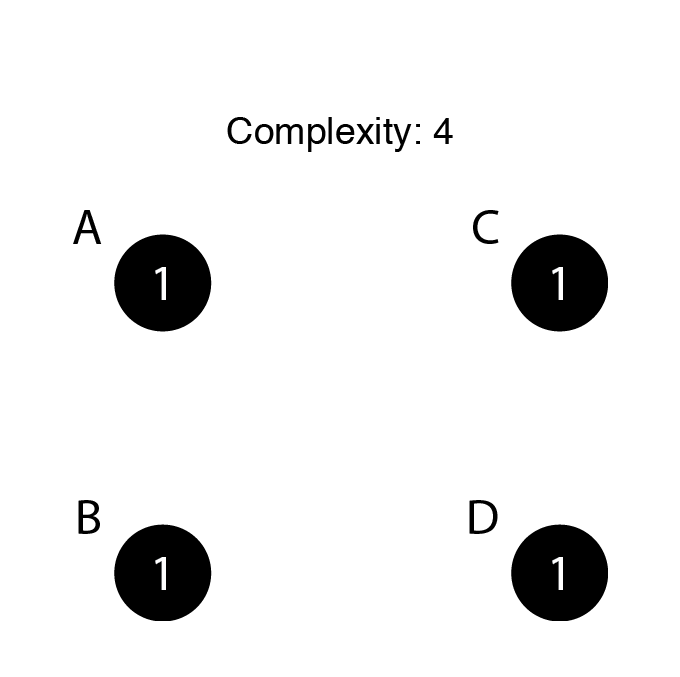
\includegraphics[width=\linewidth]{./figures/Simple4.png}
        \caption{Curriculum One}\label{fig:simple4}
      \end{subfigure}
      \begin{subfigure}[h!]{.3\linewidth}
        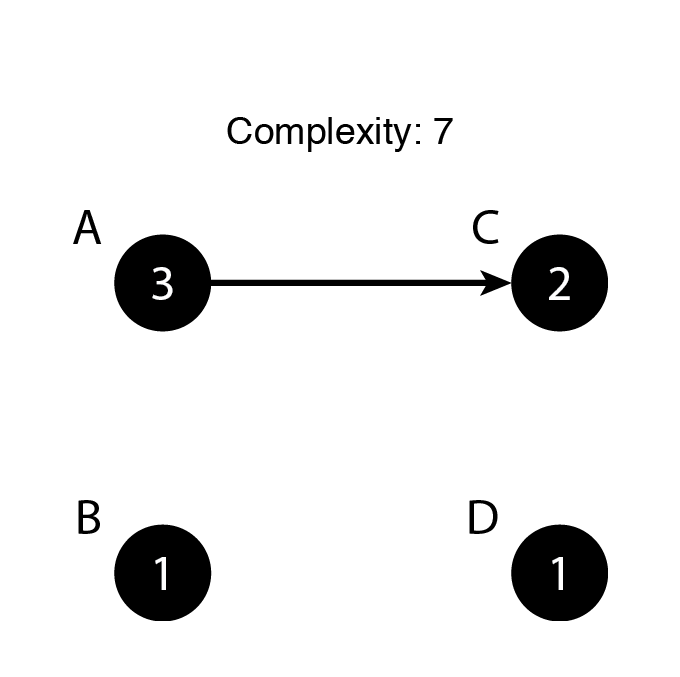
\includegraphics[width=\linewidth]{./figures/Simple7.png}
        \caption{Curriculum Two}\label{fig:simple7}
      \end{subfigure}
      \begin{subfigure}[h!]{.3\linewidth}
        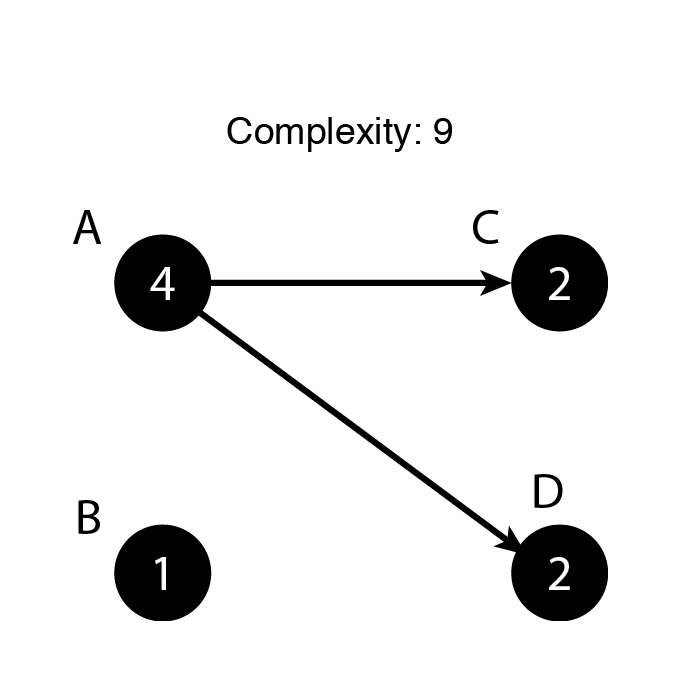
\includegraphics[width=\linewidth]{./figures/Simple9-1.png}
        \caption{Curriculum Three}\label{fig:simple91}
      \end{subfigure}

      \begin{subfigure}[h!]{.3\linewidth}
        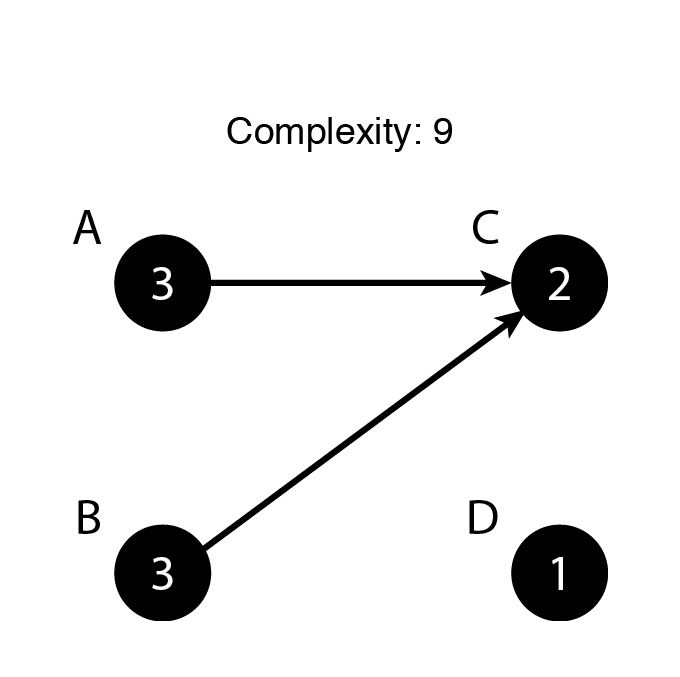
\includegraphics[width=\linewidth]{./figures/Simple9-2.png}
        \caption{Curriculum Four}\label{fig:simple92}
      \end{subfigure}
      \begin{subfigure}[h!]{.3\linewidth}
        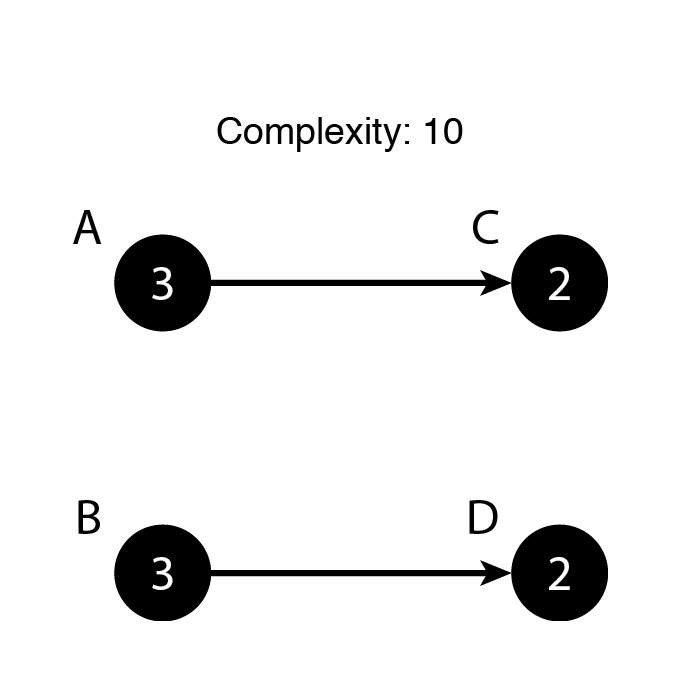
\includegraphics[width=\linewidth]{./figures/Simple10.png}
        \caption{Curriculum Five}\label{fig:simple10}
      \end{subfigure}

      \caption{Basic Curricula}
      \label{fig:simple}
    \end{figure}

    For each of these curricula, a series of one hundred simulations were run with one hundred students each where each simulation had the following parameters: 
    (1) Every courses had a 50\% pass-rate, giving each student a one in two chance of passing the course. (2) Each student could take up to three courses a term. (3) A duration of four terms.
    The results of each set of simulations were averaged together and can be seen in table \ref{tab:simpleResults}

    \begin{table}[!h]
      \tiny
      \caption{}
      \begin{subtable}{0.45\linewidth}
        \centering
          \caption{Curriculum One}
          \label{tab:simple4}
          \begin{tabular}{l*{4}{c}}
            Course  & Term 1 & Term 2 & Term 3 & Term 4 \\
            \hline
            A       & 49.62 & 75.2  & 87.33 & 93.73 \\
            B       & 50.64 & 75.48 & 87.64 & 93.97 \\
            C       & 49.98 & 75.62 & 87.98 & 94.14 \\
            D       & 0.0 & 44.1 & 71.89 & 85.77 \\
            \hline
            Completion \\ Rate & 0.0 & 20.72 & 49.5 & 71.63
          \end{tabular}
      \end{subtable}\hfill
      \begin{subtable}{0.45\linewidth}
        \centering
          \caption{Curriculum Two}
          \label{tab:simple7}
          \begin{tabular}{l*{4}{c}}
            Course  & Term 1 & Term 2 & Term 3 & Term 4 \\
            \hline
            A       & 51.19 & 75.31 & 87.23 & 93.48 \\
            B       & 49.94 & 74.71 & 87.31 & 93.45 \\
            C       & 0.0   & 25.5  & 51.27 & 69.39 \\
            D       & 49.3  & 75.2  & 87.31 & 93.59 \\
            \hline
            Completion \\ Rate & 0.0 & 14.35 & 39.21 & 60.41 \\
          \end{tabular}
      \end{subtable}

      \vspace*{1cm}
      \begin{subtable}{0.45\linewidth}
        \centering
          \caption{Curriculum Three}
          \label{tab:simple91}
          \begin{tabular}{l*{4}{c}}
            Course  & Term 1 & Term 2 & Term 3 & Term 4 \\
            \hline
            A & 49.96 & 74.78 & 87.43 & 93.38 \\
            B & 49.68 & 74.57 & 87.28 & 93.95 \\
            C & 0.0   & 25.59 & 50.51 & 69.2  \\
            D & 0.0   & 24.61 & 49.64 & 68.83 \\
            \hline
            Completion \\ Rate & 0.0   & 8.88  & 30.01 & 52.57 \\
          \end{tabular}
      \end{subtable} 
      \hfill
      \begin{subtable}{0.45\linewidth}
        \centering
          \caption{Curriculum Four}
          \label{tab:simple92}
          \begin{tabular}{l*{4}{c}}
            Course  & Term 1 & Term 2 & Term 3 & Term 4 \\
            \hline
            A & 49.98 & 75.12 & 87.93 & 93.92 \\
            B & 49.76 & 75.44 & 87.37 & 93.73 \\
            C & 0.0   & 12.35 & 34.7  & 55.21 \\
            D & 49.98 & 75.4  & 87.79 & 94.33 \\
            \hline
            Completion \\ Rate & 0.0   & 9.31  & 30.44 & 52.3  \\
          \end{tabular}
      \end{subtable}

      \vspace*{1cm}
      \begin{subtable}{0.45\linewidth}
        \centering
          \caption{Curriculum Five}
          \label{tab:simple10}
          \begin{tabular}{l*{4}{c}}
            Course  & Term 1 & Term 2 & Term 3 & Term 4 \\
            \hline
            A & 49.9  & 74.99 & 87.75 & 93.6  \\
            B & 49.93 & 75.1  & 88.0  & 94.05 \\
            C & 0.0   & 25.21 & 50.07 & 68.75 \\
            D & 0.0   & 24.61 & 49.47 & 68.61 \\
            \hline
            Completion \\ Rate & 0.0   & 6.07  & 24.5  & 46.93 \\
          \end{tabular}
      \end{subtable} 
      \label{tab:simpleResults}
    \end{table}

    These tables give insights into how students progress through a curriculum by showing the percentage of students that have passed each course at the end of each semester. For example, looking at table \ref{tab:simple4}, 75.2\% of students have passed Course A after the second term. The row at the bottom shows the percentage of students that have completed all courses (ie graduated) at the end of each term. As expected, the least complex curriculum had the highest completion rate after four terms, while the most complexity curricula had the lowest completion rate. It is also interesting, though not surprising, that the two curricula with the same complexity had roughly the same fourth term completion rate even though their structures were different.

    To expand upon the previous experiment similar simulations were conducted over slightly more complex curricula with an additional term consisting of two courses for a total of 6 courses. Even with the addition of only two courses, the number of structures greatly increases providing a much larger curricula set with a wider range of complexities. In total 256 curricula systematically generated with the three terms, six courses specification. For each generated curricula, simulations similar to those done with the simple curricula were carried with slightly different parameters: (1) Every courses had a 80\% pass-rate. (2) Each student can take up to three courses a term. (3) A duration of five terms. The results of these simulation can be seen in figure \ref{fig:gen6results}.

    \begin{figure}[h!]
      \centerline{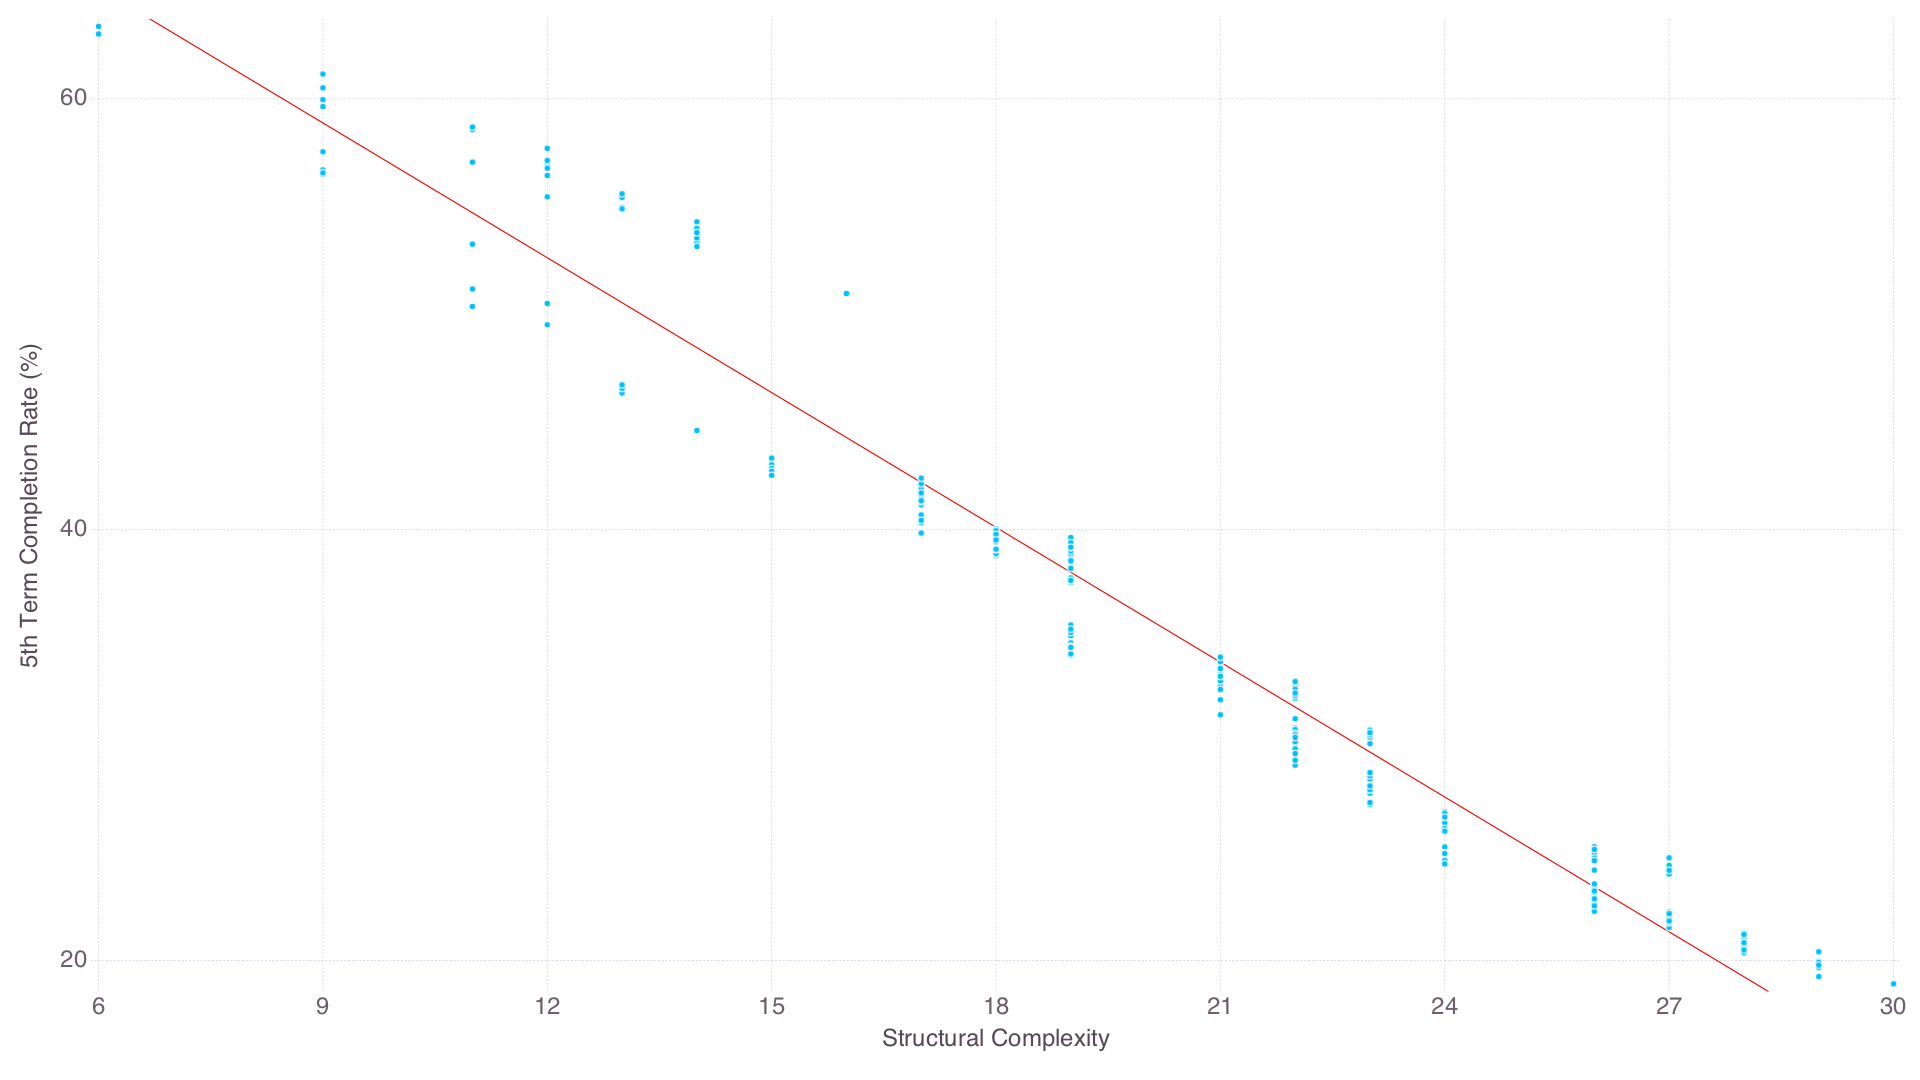
\includegraphics[scale=0.25]{./figures/gradRate5_v_Complexity.png}}
      \caption{A plot of complexity vs 5th term graduation rates for six course curricula.} 
      \label{fig:gen6results}
    \end{figure}

    Again, the results imply a correlation between structure and completion rates. To more formally characterize this correlation, linear regression was performed over the data, the details of which can be seen in table \ref{tab:gen6reg} and is visualized by the red line in figure \ref{fig:gen6results}. The R-Squared value is a 95.8\%. Based on this regression, for every point of complexity added, the fith-term completion rate will decrease by 2\%, which is fairly significant. While these results are good, they are not perfect. Unlike the results from the four-course curricula where the two with the same complexity resulted in the same completion rates, introducing two more courses also introduces more variance between completion rates of same-complexity curricula.

    \begin{table}[!h]
      \centering
      \caption{Six-Course Curricula Linear Regression Results}
      \label{tab:gen6reg}
      \begin{tabular}{l*{4}{c}}
        Coefficient & Estimate  & Std Error & Z Value & Pr(>|z|) \\
        \hline
        (Intercept) & 77.66     & 0.57      & 137.04  & <1e-99 \\
        Complexity  & -2.09     & 0.027     & -76.73  & <1e-99 \\
      \end{tabular}
    \end{table}

    The final set of experiments were conducted over real-world curricula pulled from \href{http://curricula.academicdashboards.org}{curricula.academicdashboards.org}, a web service that stores, visualizes and computes the complexity of curricula. It hosts overs 120 curricula from Universities around that country, and pulling those that have at least eight terms and between 100 and 150 credit hours results in a set of thirty eight curricula. These curricula are then simulated 50 times each with 1000 students using the parameters: (1) Every courses had a 80\% pass-rate. (2) Each student can take up to eighteen credit hours a term. (3) A duration of ten terms. A plot of the results can be seen in figure \ref{fig:web10}. 

    \begin{figure}[h!]
      \centerline{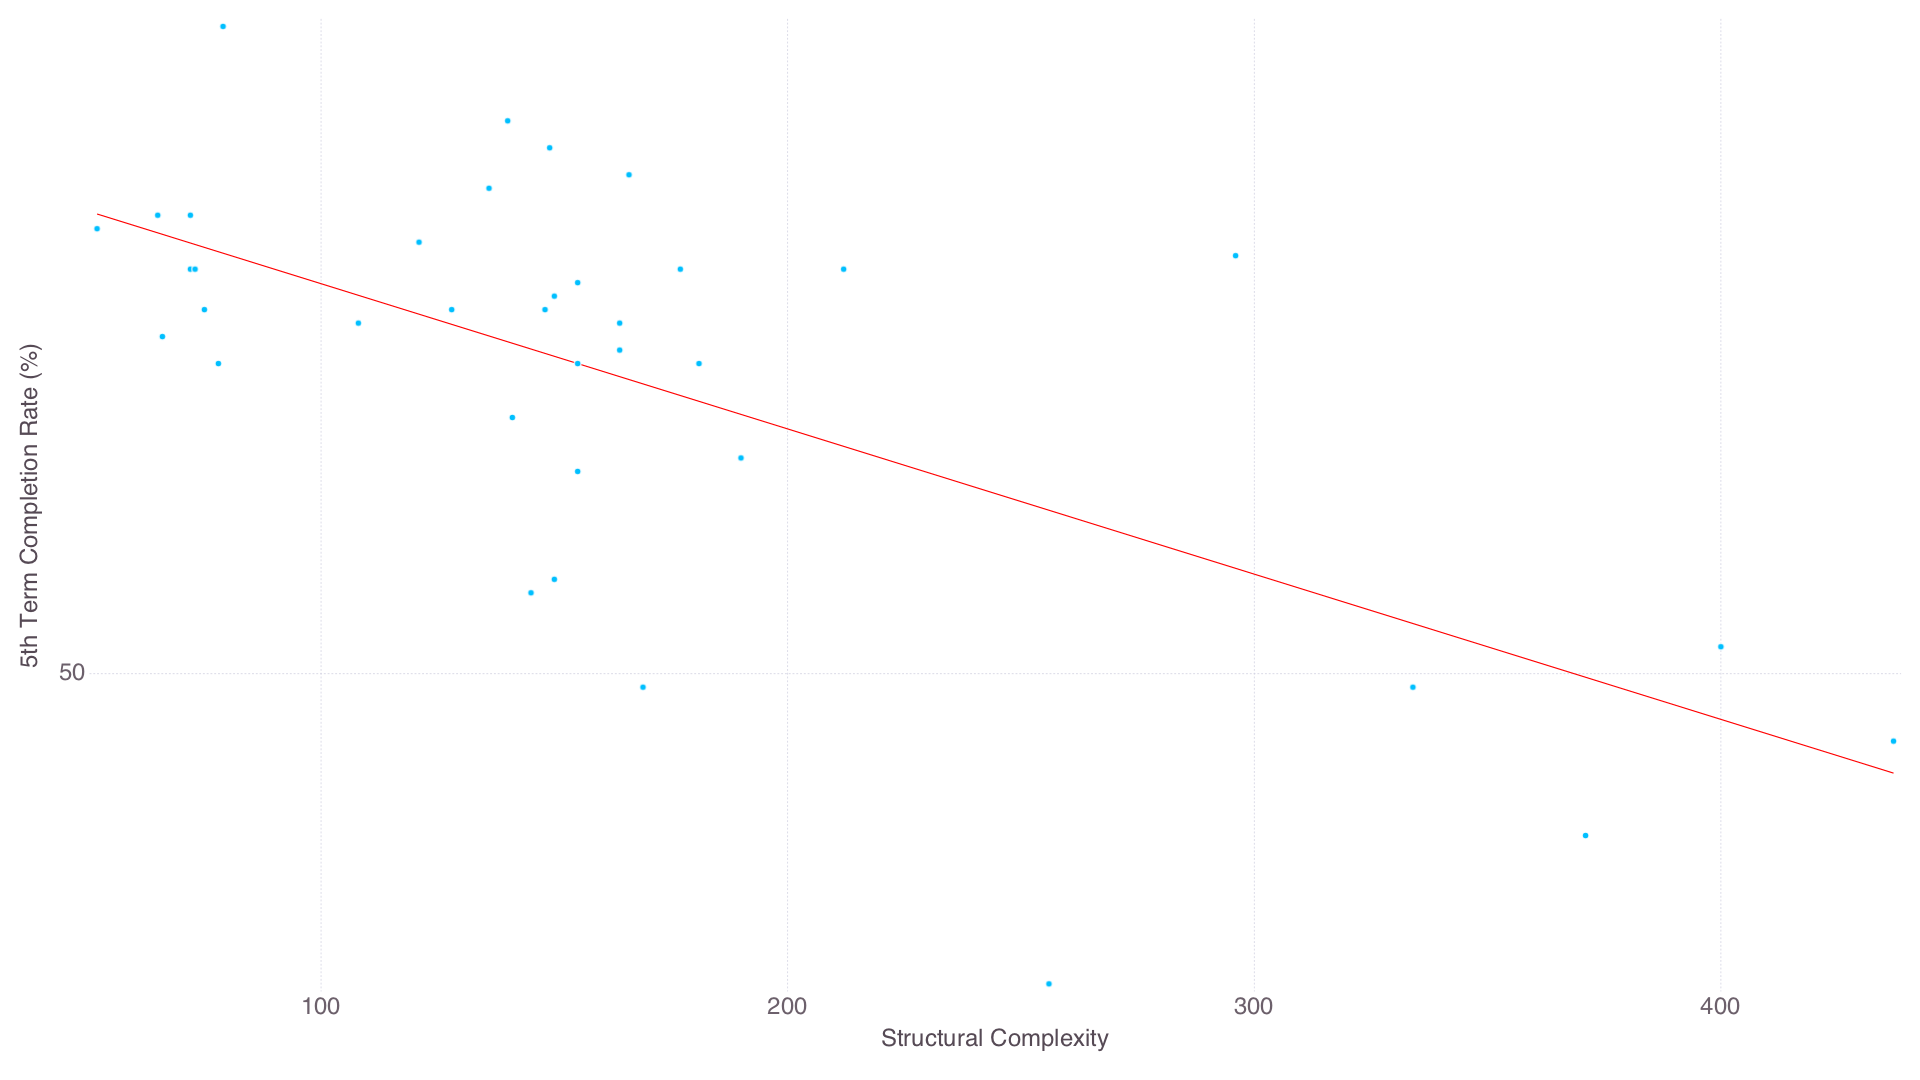
\includegraphics[scale=0.25]{./figures/gradRate10_v_complexity.png}}
      \caption{Simulation results of thirty eight real-world curricula.} 
      \label{fig:web10}
    \end{figure}

    Like the two experiments before, an inverse relationship exists between complexity and completion rates, however here there is much more variance. Again linear regression was employed, indicated by the red line, and it is easy to see that there is not as tight of a fit to the results as there was with the six-course curriculum. This is indicated in the resulting R-Squared value of 0.438. This is fairly unsurprising given the more varied nature of the real-world curricula, however there might be other issues that affect this relationship. For example, the previous two experiments used sets of curricula that had the same number of courses and therefore the same number of credit hours. This is not the case with the real-world curricula which span a range of 100 to 150 credit hours. To try and account for this, another regression was performed with credit hours being a independent variable. The results of this regression can be seen in table \ref{tab:webCH} and is visualized in figure \ref{fig:wbcompch}. It is easy to see that this change produces a much tighter, though not perfect, fit with a R-Squared value of 0.703.

    \begin{table}[!h]
      \centering
      \caption{Real-World curricula regression results using complexity and credit hours as variables.}
      \label{tab:webCH}
      \begin{tabular}{l*{4}{c}}
        Coefficient   & Estimate    & Std Error & Z Value   & Pr(>|z|)  \\
        \hline
        (Intercept)   & 255.169     & 29.748    & 8.57771   & <1e-17    \\
        complexity    & -0.0882544  & 0.0154001 & -5.73077  & <1e-8     \\
        credit hours  & -1.38057    & 0.24707   & -5.58778  & <1e-7     \\
      \end{tabular}
    \end{table}

    \begin{figure}[h!]
      \centerline{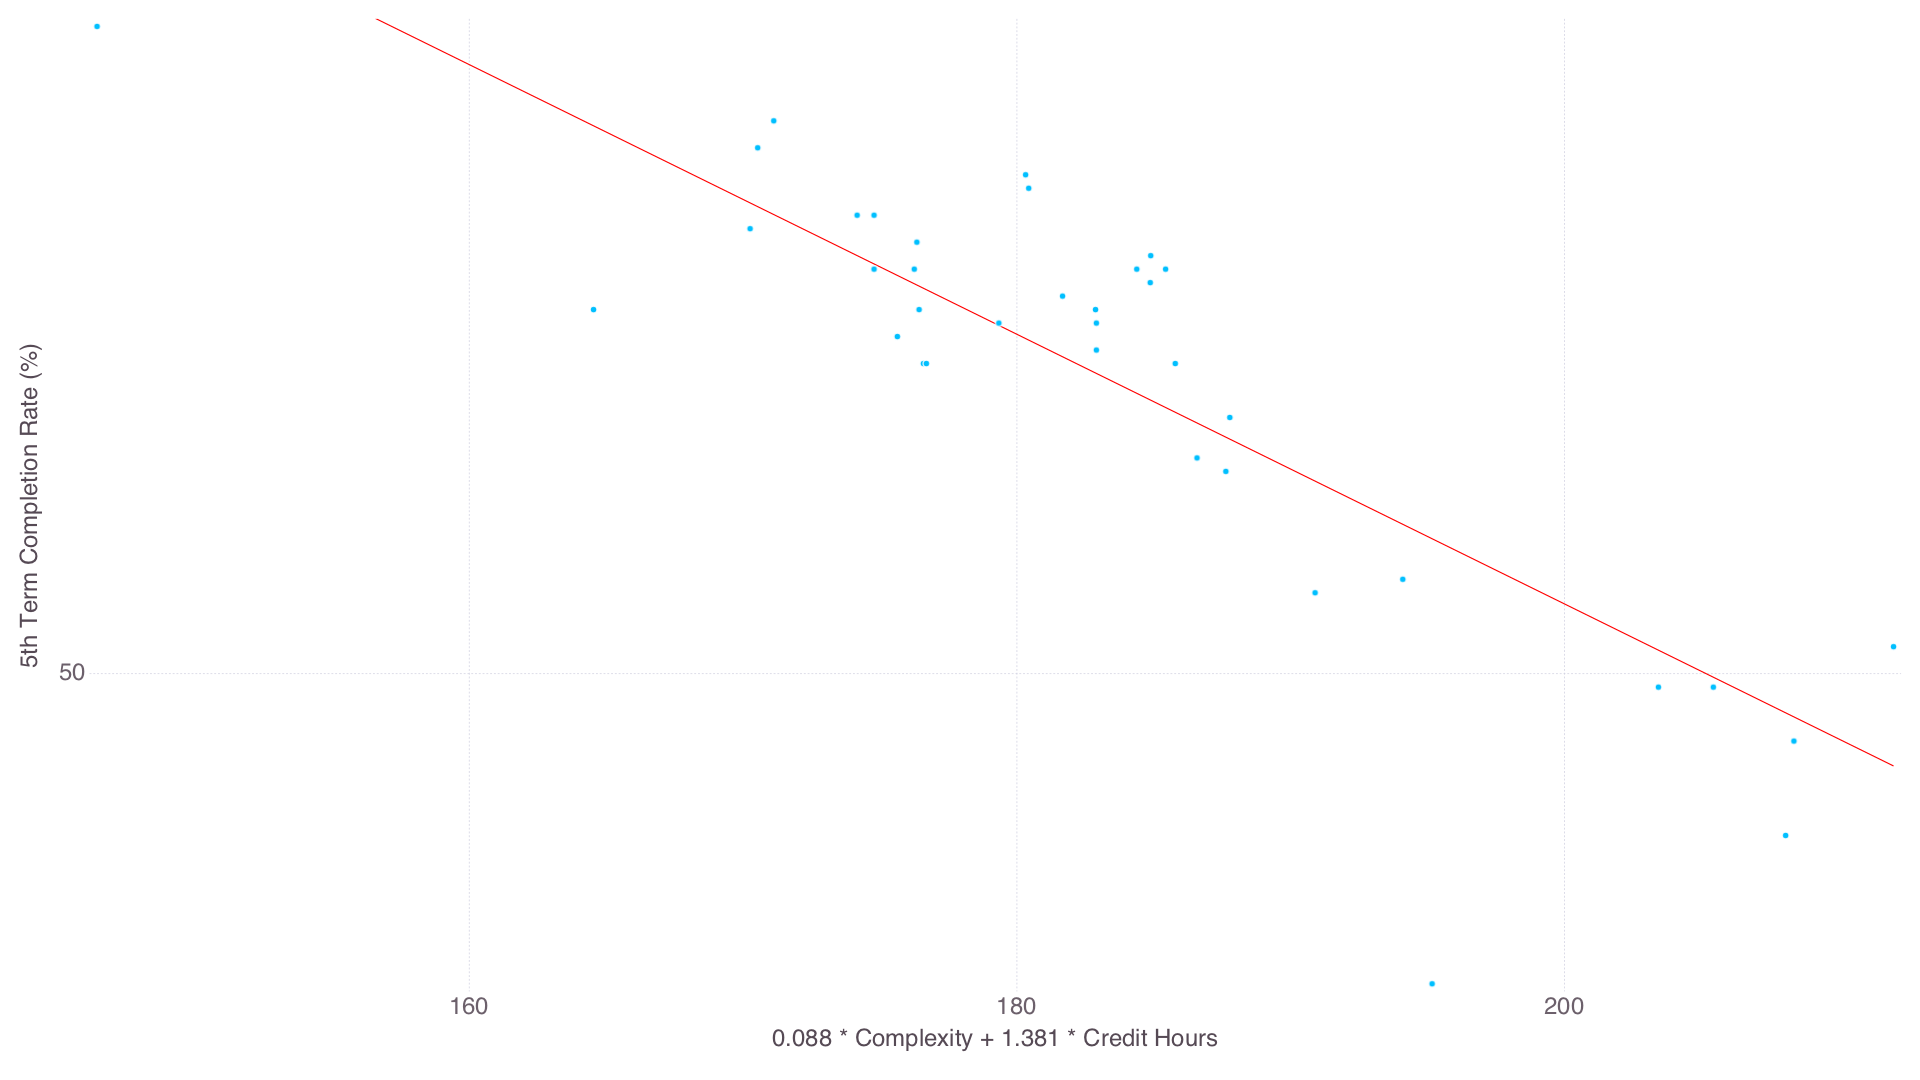
\includegraphics[scale=0.25]{./figures/comp_ch_plot.png}}
      \caption{Real-World curricula regression analysis using complexity and credit hours as variables.} 
      \label{fig:wbcompch}
    \end{figure}


  \section{Evaluating Complexity Measures}  
    TODO: Include evaluation of centrality and reachability with regression results.


  \section{Sensitivity Analysis of Instructional Complexity}
    Another metric that is useful when working with curricula is the instructional complexity of a curriculum. This can be thought of as the difficulty of the curriculum, which in term will be defined by the difficulty of the courses that make it up. Defining how difficulty a course is not straightforward and can be done in many ways, but in the experiments described here, the naive definition of the course's pass-rate is used. Another use of the curriculum flow simulation framework is to observe the effects that instructional complexity has, as it is intuitive to believe that the difficulty of a curriculum's courses would greatly affect student performance. Although not a realistic scenario, Figure \ref{fig:instructional} illustrates this point.

    \begin{figure}[h!]
      \centerline{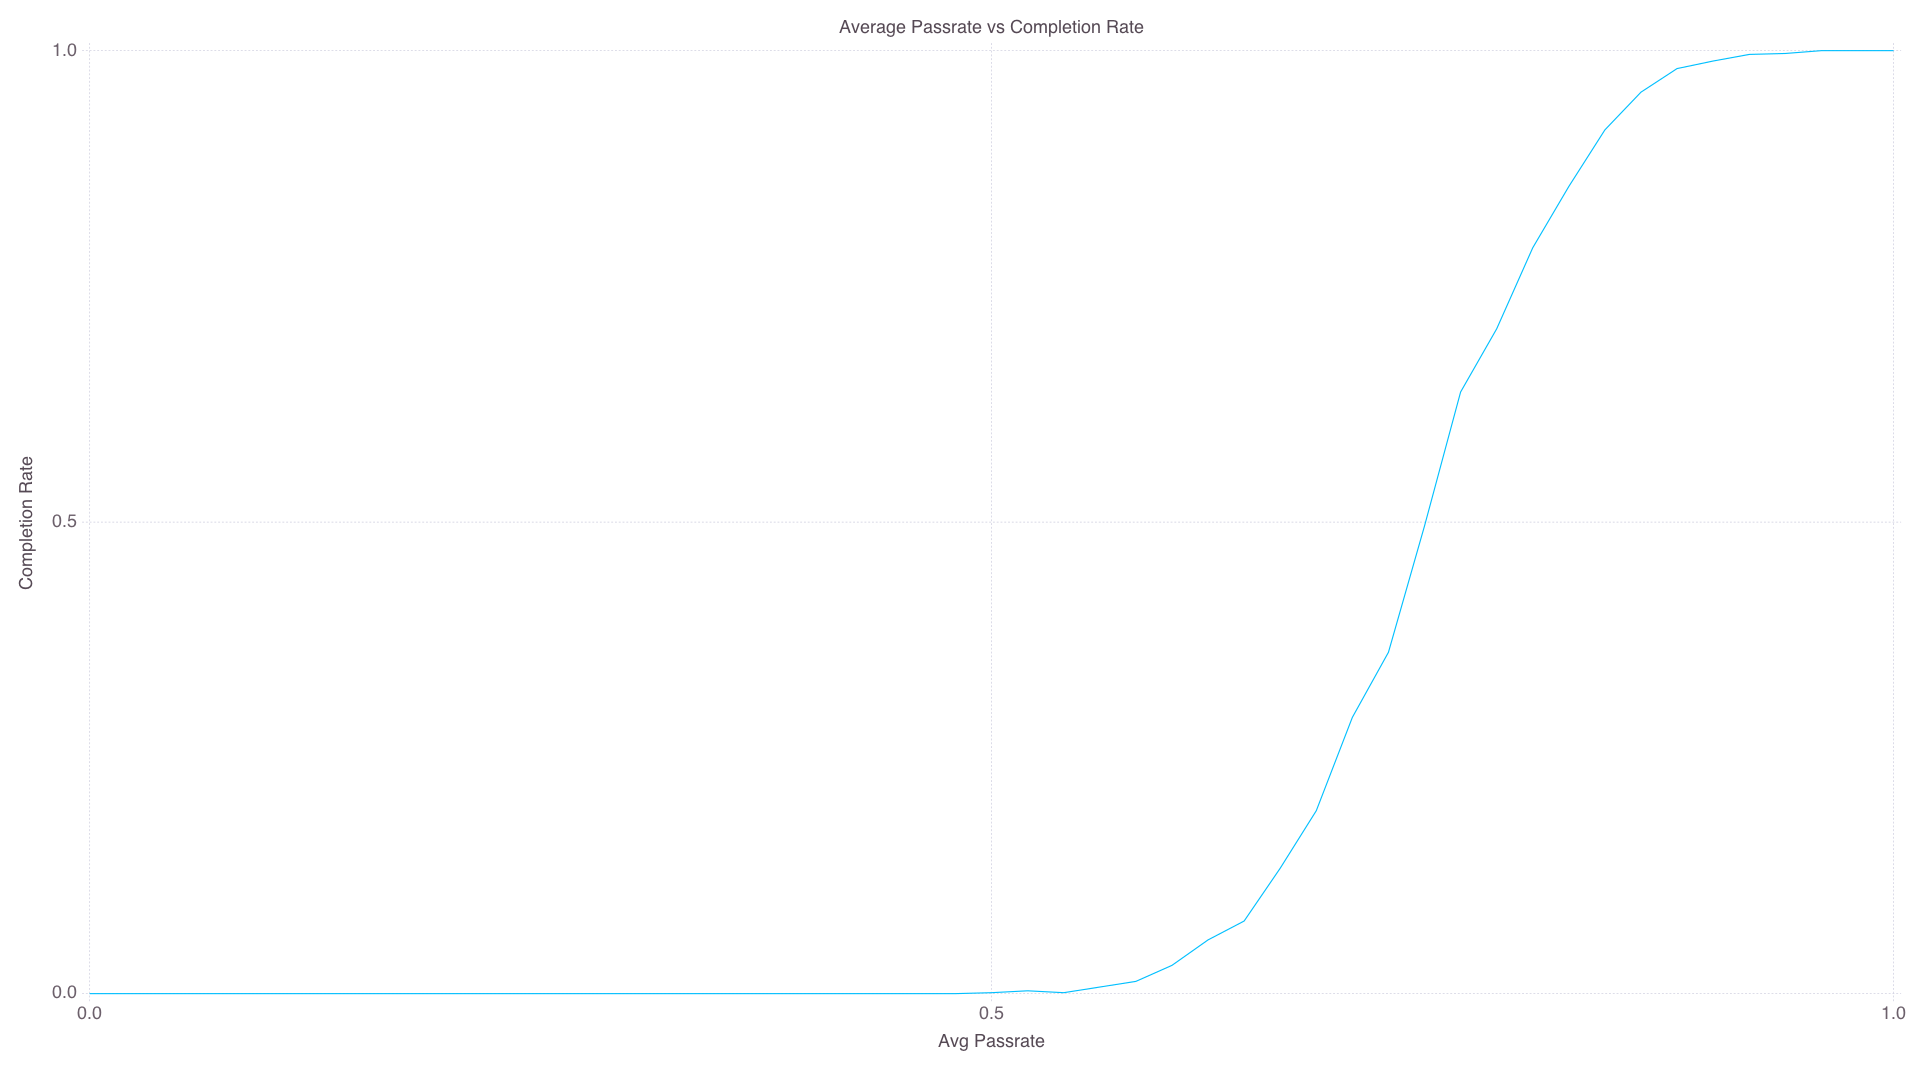
\includegraphics[scale=0.2]{./figures/instructional.png}}
      \caption{Graph showing how the completion rate of the Computer Engineering curriculum at UNM changes with respect to course pass-rates.} 
      \label{fig:instructional}
    \end{figure}

    This figure shows the completion rate of the Computer Engineering curriculum for a given pass-rate assigned to every course. As expected, the completion rates increase as course pass-rates increase and shows how the instructional complexity of a curriculum affects student success. One of the most common methods for increasing student success is to increase student success in individual courses. Regardless of the method used, increasing the pass-rate of critical courses can increase student graduation rates. So then the question becomes which courses should receive the most attention?

    This question can be answered by performing sensitivity analysis over course pass-rates via simulation. This analysis is done by performing a baseline simulation and then increasing a course's pass-rate and then measuring the difference. This experiment was carried out over three UNM curricula, Computer Engineering, Accounting, and Mechanical Engineering, where pass-rates of every were computed using UNM data over the last ten years. To get a baseline completion rate, a simulation over 1000 students was carried out 20 times and then the eighth term completion rates were averaged. Then, one at a time, each course's pass-rate is increased up to thirty percent and then an identical simulation was carried out. Figures \ref{tab:accounting_sensitivity}, \ref{tab:me_sensitivity}, and \ref{tab:cpe_sensitivity} show the results of this analysis - specifically the top 10 courses in which an increase in pass-rate had the greatest affect on eighth-term completion rates.

    \begin{table}[!h]
    \tiny
    \begin{tabular}{l*{4}{c}}
    Course & Original Pass-rate & Increased Pass-rate & Cruciality & Increase in Completion Rate \\
    \hline
    Elective & 0.9 & 1 & 1 & 0.0836 \\
    MATH 180 & 0.7397 & 0.9616 & 4 & 0.0282 \\
    MGMT 202 & 0.8038 & 1 & 12 & 0.028 \\
    MATH 121 & 0.7389 & 0.9606 & 10 & 0.0274 \\
    ECON 105 & 0.7904 & 1 & 1 & 0.0227 \\
    ECON 106 & 0.7984 & 1 & 8 & 0.0224 \\
    MGMT 340 & 0.8943 & 1 & 6 & 0.0154 \\
    MGMT 326 & 0.8605 & 1 & 3 & 0.0147 \\
    Foreign Language & 0.9 & 1 & 1 & 0.0142 \\
    Physical \& Natural Science & 0.9 & 1 & 1 & 0.0139 \\
    \end{tabular}
    \caption{Accounting Sensitivity Analysis} 
    \label{tab:accounting_sensitivity}
    \end{table}

    \begin{table}[!h]
    \tiny
    \begin{tabular}{l*{4}{c}}
    Course & Original Pass-rate & Increased Pass-rate & Cruciality & Increase in Completion Rate \\
    \hline
    MATH 162 & 0.7585 & 0.9861 & 29 & 0.0407 \\
    MATH 163 & 0.7502 & 0.9753 & 26 & 0.0404 \\
    MATH 264 & 0.8399 & 1 & 16 & 0.0265 \\
    PHYC 160 & 0.7926 & 1 & 25 & 0.0212 \\
    ECON 105 & 0.7904 & 1 & 1 & 0.0206 \\
    Tech Elective & 0.9 & 1 & 1 & 0.0195 \\
    Tech Elective & 0.9 & 1 & 1 & 0.0163 \\
    CHEM 121 & 0.8049 & 1 & 13 & 0.0158 \\
    Tech Elective & 0.9 & 1 & 1 & 0.0143 \\
    MATH 316 & 0.8633 & 1 & 18 & 0.0108 \\
    \end{tabular}
    \caption{Mechanical Engineering Sensitivity Analysis}
    \label{tab:me_sensitivity}
    \end{table}

    \begin{table}[!h]
    \tiny
    \begin{tabular}{l*{4}{c}}
    Course & Original Pass-rate & Increased Pass-rate & Cruciality & Increase in Completion Rate \\
    \hline
    Humanities & 0.9 & 1 & 1 & 0.0661 \\
    MATH 162 & 0.7585 & 0.9861 & 19 & 0.0609 \\
    MATH 163 & 0.7502 & 0.9753 & 18 & 0.0554 \\
    Fine Arts & 0.9 & 1 & 1 & 0.0474 \\
    Tech Elective & 0.9 & 1 & 1 & 0.0396 \\
    PHYC 160 & 0.7926 & 1 & 14 & 0.0287 \\
    MATH 264 & 0.8399 & 1 & 5 & 0.0251 \\
    ECON 105 & 0.7904 & 1 & 1 & 0.0239 \\
    ECE 344L & 0.9026 & 1 & 6 & 0.0237 \\
    ECE 131 & 0.8571 & 1 & 13 & 0.0218 \\
    \end{tabular}
    \caption{Computer Engineering Sensitivity Analysis}
    \label{tab:cpe_sensitivity}
    \end{table}

    In each curricula, the courses with the highest cruciality had some of the greatest increases in completion rates with an increase in their pass-rates. This makes sense as these are courses are on long-paths and block other crucial courses. 

%----------------------------------------------------------------------------------------
%  Discussion
%----------------------------------------------------------------------------------------
\chapter{Discussion}
TODO

%----------------------------------------------------------------------------------------
%  Future Work
%----------------------------------------------------------------------------------------
\chapter{Future Work}
TODO

%----------------------------------------------------------------------------------------
%  REFERENCE LIST
%----------------------------------------------------------------------------------------
\vspace{4\baselineskip}\vspace{-\parskip} % Creaters proper 4 blank line spacing.
\footnotesize % Makes bibliography 10 pt font.
\bibliographystyle{abbrv} %Can use a different style as long as it is one which uses numbered references in the text.
\bibliography{thesis}

\end{document}
